%% Modelo adaptado de abtex2-modelo-trabalho-academico.tex, v-1.8 laurocesar
%% Copyright 2012-2013 by abnTeX2 group at http://abntex2.googlecode.com/ 
%%
%% This work may be distributed and/or modified under the
%% conditions of the LaTeX Project Public License, either version 1.3
%% of this license or (at your option) any later version.
%% The latest version of this license is in
%%   http://www.latex-project.org/lppl.txt
%% and version 1.3 or later is part of all distributions of LaTeX
%% version 2005/12/01 or later.
%%
%% This work has the LPPL maintenance status `maintained'.
%% 
%% The Current Maintainer of this work is the abnTeX2 team, led
%% by Lauro César Araujo. Further information are available on 
%% http://abntex2.googlecode.com/

%%******************************************************
%%******************************************************
%% This work consists of the files:
%% abntex2-modelo-trabalho-academico-TCC-EngaEletrica.tex,
%% abntex2-modelo-include-comandos 
%% abntex2-modelo-references.bib
%%******************************************************
%%******************************************************

% ------------------------------------------------------------------------
% ------------------------------------------------------------------------
% abnTeX2: Modelo de Trabalho Academico (tese de doutorado, dissertacao de
% mestrado e trabalhos monograficos em geral) em conformidade com 
% ABNT NBR 14724:2011: Informacao e documentacao - Trabalhos academicos -
% Apresentacao
% ------------------------------------------------------------------------
% ------------------------------------------------------------------------

\documentclass[
	% -- opções da classe memoir --
	12pt,				% tamanho da fonte
	% openright,			% capítulos começam em pág ímpar (insere página vazia caso preciso)
	openany,
	onseside,
	%twoside,			% para impressão em verso e anverso. Oposto a oneside
	a4paper,			% tamanho do papel. 
	% -- opções da classe abntex2 --
	%chapter=TITLE,		% títulos de capítulos convertidos em letras maiúsculas
	%section=TITLE,		% títulos de seções convertidos em letras maiúsculas
	%subsection=TITLE,	% títulos de subseções convertidos em letras maiúsculas
	%subsubsection=TITLE,% títulos de subsubseções convertidos em letras maiúsculas
	% -- opções do pacote babel --\usepackage[bottom]{footmisc}
	english,			% idioma adicional para hifenização
	french,				% idioma adicional para hifenização
	spanish,			% idioma adicional para hifenização
	brazil,				% o último idioma é o principal do documento
	]{abntex2}


% ---
% PACOTES
% ---

% ---
% Pacotes fundamentais 
% ---
\usepackage{cmap}			% Mapear caracteres especiais no PDF
\usepackage{lmodern}			% Usa a fonte Latin Modern			
\usepackage[T1]{fontenc}		% Selecao de codigos de fonte.
\usepackage[utf8]{inputenc}		% Codificacao do documento (conversão automática dos acentos)
\usepackage{lastpage}			% Usado pela Ficha catalográfica
\usepackage{indentfirst}		           % Indenta o primeiro parágrafo de cada seção.
\usepackage{color}				% Controle das cores
\usepackage{graphicx}			% Inclusão de gráficos
% ---

\graphicspath{{images/}}

\usepackage{amsmath}
\usepackage{IEEEtrantools}
\usepackage{subfig}
\usepackage[table,xcdraw]{xcolor}
\usepackage[bottom]{footmisc}
\usepackage{listings}
\usepackage[figuresright]{rotating}
\usepackage{float}
\usepackage{multirow}

% ---
% Pacotes adicionais, usados apenas no âmbito do Modelo Canônico do abnteX2
% ---
\usepackage{lipsum}			% para geração de dummy text
% ---

% ---
% Pacotes de citações
% ---
\usepackage[brazilian,hyperpageref]{backref}   % Paginas com as citações na bibl
\usepackage[alf]{abntex2cite}	                         % Citações padrão ABNT




% --- 
% CONFIGURAÇÕES DE PACOTES
% --- 

% ---
% Configurações do pacote backref
% Usado sem a opção hyperpageref de backref
\renewcommand{\backrefpagesname}{Citado na(s) página(s):~}
% Texto padrão antes do número das páginas
\renewcommand{\backref}{}
% Define os textos da citação
\renewcommand*{\backrefalt}[4]{
	\ifcase #1 %
		Nenhuma citação no texto.%
	\or
		Citado na página #2.%
	\else
		Citado #1 vezes nas páginas #2.%
	\fi}%



	\usepackage{xpatch}
	\xpatchbibdriver{online}
  {\printtext[parens]{\usebibmacro{date}}}
  {\iffieldundef{year}{}{\printtext[parens]{\usebibmacro{date}}}}
  {}{}
% ---


% ---
% Informações de dados para CAPA e FOLHA DE ROSTO
% ---
\titulo{Estudo de Microinversores Baseados no Conversor Ćuk Para Painéis Fotovoltaicos Conectados à Rede Elétrica}
\autor{Raul Henrique Santana}
\local{Belo Horizonte}
\data{2019}
\orientador{Prof. Pedro Francisco Donoso-Garcia}
%\coorientador{Prof. }
\instituicao{%
  Universidade Federal de Minas Gerais -- UFMG
  \par
  Escola de Engenharia
  \par
  Curso de Graduação em Engenharia Elétrica}
\tipotrabalho{Trabalho de Conclusão de Curso}

% O preambulo deve conter o tipo do trabalho, o objetivo, o nome da instituição e a área de concentração 
\preambulo{Monografia apresentada durante o Seminário dos Trabalhos de Conclusão do Curso de Graduação em Engenharia Elétrica da UFMG, como parte dos requisitos necessários à obtenção do título de Engenheiro Eletricista.}
% ---

% ---
% Configurações de aparência do PDF final

% alterando o aspecto da cor azul
\definecolor{blue}{RGB}{41,5,195}

% informações do PDF
\makeatletter
\hypersetup{
     	%pagebackref=true,
		pdftitle={\@title}, 
		pdfauthor={\@author},
    	pdfsubject={\imprimirpreambulo},
	    pdfcreator={LaTeX with abnTeX2},
		pdfkeywords={abnt}{latex}{abntex}{abntex2}{trabalho acadêmico}, 
		colorlinks=true,       	% false: boxed links; true: colored links
    	linkcolor=blue,          	           % color of internal links
    	citecolor=blue,        		% color of links to bibliography
    	filecolor=magenta,      		% color of file links
		urlcolor=blue,
		bookmarksdepth=4
}
\makeatother
% --- 

% --- 
% Espaçamentos entre linhas e parágrafos 
% --- 

% O tamanho do parágrafo é dado por:
\setlength{\parindent}{1.3cm}

% Controle do espaçamento entre um parágrafo e outro:
\setlength{\parskip}{0.2cm}  % tente também \onelineskip

% ---
% compila o indice
% ---
\makeindex
% ---

% ----
% Início do documento
% ----
\begin{document}

% Retira espaço extra obsoleto entre as frases.
\frenchspacing 

% ----------------------------------------------------------
% ELEMENTOS PRÉ-TEXTUAIS
% ----------------------------------------------------------
% \pretextual

% ---
% Capa
% ---
\imprimircapa
% ---

% ---
% Folha de rosto
% ---
\imprimirfolhaderosto
% ---

% ---
% Dedicatória
% ---
\begin{comment}


	\begin{dedicatoria}
	   \vspace*{\fill}
	   \centering
	   \noindent
	   \textit{ Este trabalho é dedicado às crianças adultas que,\\
	   quando pequenas, sonharam em se tornar cientistas.} \vspace*{\fill}
	\end{dedicatoria}

\end{comment}
% ---

% ---
% Agradecimentos
% ---

\begin{comment}

	\begin{agradecimentos}
	Os agradecimentos principais são direcionados à Gerald Weber, Miguel Frasson,
	Leslie H. Watter, Bruno Parente Lima, Flávio de Vasconcellos Corrêa, Otavio Real
	Salvador, Renato Machnievscz\footnote{Os nomes dos integrantes do primeiro
	projeto abn\TeX\ foram extraídos de
	\url{http://codigolivre.org.br/projects/abntex/}} e todos aqueles que
	contribuíram para que a produção de trabalhos acadêmicos conforme
	as normas ABNT com \LaTeX\ fosse possível.

	Agradecimentos especiais são direcionados ao Centro de Pesquisa em Arquitetura
	da Informação\footnote{\url{http://www.cpai.unb.br/}} da Universidade de
	Brasília (CPAI), ao grupo de usuários
	\emph{latex-br}\footnote{\url{http://groups.google.com/group/latex-br}} e aos
	novos voluntários do grupo
	\emph{\abnTeX}\footnote{\url{http://groups.google.com/group/abntex2} e
	\url{http://abntex2.googlecode.com/}}~que contribuíram e que ainda
	contribuirão para a evolução do \abnTeX.
	\end{agradecimentos}

\end{comment}
% ---

% ---
% Epígrafe
% ---
\begin{comment}


	\begin{epigrafe}
			\vspace*{\fill}
		\begin{flushright}
			\textit{``Não vos amoldeis às estruturas deste mundo, \\
			mas transformai-vos pela renovação da mente, \\
			a fim de distinguir qual é a vontade de Deus: \\
			o que é bom, o que Lhe é agradável, o que é perfeito.\\
			(Bíblia Sagrada, Romanos 12, 2)}
		\end{flushright}
	\end{epigrafe}

\end{comment}
% ---

% ---
% RESUMOS
% ---
% resumo em português
\begin{comment}

	\setlength{\absparsep}{18pt} % ajusta o espaçamento dos parágrafos do resumo
	\begin{resumo}
	Segundo a \citeonline[3.1-3.2]{NBR6028:2003}, o resumo deve ressaltar o
	objetivo, o método, os resultados e as conclusões do documento. A ordem e a extensão
	destes itens dependem do tipo de resumo (informativo ou indicativo) e do
	tratamento que cada item recebe no documento original. O resumo deve ser
	precedido da referência do documento, com exceção do resumo inserido no
	próprio documento. (\ldots) As palavras-chave devem figurar logo abaixo do
	resumo, antecedidas da expressão Palavras-chave:, separadas entre si por
	ponto e finalizadas também por ponto.

	\textbf{Palavras-chaves}: latex. abntex. editoração de texto.
	\end{resumo}

	% resumo em inglês
	\begin{resumo}[Abstract]
	\begin{otherlanguage*}{english}
		This is the english abstract.

		\vspace{\onelineskip}
	
		\noindent 
		\textbf{Key-words}: latex. abntex. text editoration.
	\end{otherlanguage*}
	\end{resumo}

\end{comment}

% \begin{comment}
	% ---
	% inserir lista de ilustrações
	% ---
	\pdfbookmark[0]{\listfigurename}{lof}
	\listoffigures*
	%\cleardoublepage
	\clearpage
	% ---

	% ---
	% inserir lista de tabelas
	% ---
	\pdfbookmark[0]{\listtablename}{lot}
	\listoftables*
	%\cleardoublepage
	\clearpage
	% ---

\begin{comment}
	
	% ---
	% inserir lista de abreviaturas e siglas
	% ---
	\begin{siglas}
	%   \item[Fig.] Area of the $i^{th}$ component
	%   \item[456] Isto é um número
	%   \item[123] Isto é outro número
	%   \item[lauro cesar] este é o meu nome
		\item[CA] Corrente Contínua
		\item[CC] Corrente Contínua
	    \item[SCP] Sistema de condicionamento de Potência
	    \item[PCS] \textit{Power conditioning system}
		\item[MPPT] \textit{Maximum power point tracker}

	\end{siglas}

\end{comment}

% ---
\begin{comment}

	% ---
	% inserir lista de símbolos
	% ---
	\begin{simbolos}
	  \item[$ \Gamma $] Letra grega Gama
	  \item[$ \Lambda $] Lambda
	  \item[$ \zeta $] Letra grega minúscula zeta
	  \item[$ \in $] Pertence
	\end{simbolos}
	% ---

\end{comment}

% ---
% inserir o sumario
% ---
\pdfbookmark[0]{\contentsname}{toc}
\tableofcontents*
%\cleardoublepage
%\clearpage
% ---

% ----------------------------------------------------------
% ELEMENTOS TEXTUAIS
% ----------------------------------------------------------
\textual

% ----------------------------------------------------------
% Capítulo 1 - Introdução
% ----------------------------------------------------------
\chapter{Introdução}

\section{Motivação}

	A geração de energia elétrica no Brasil é fortemente caracterizada por um modelo geração centralizada e faz uso 
	do conceito de economias de escala \cite{MACHADO2016290}.
	Nesse modelo, plantas de grande porte geram toda a energia, que é transmitida e distribuída aos
	consumidores, ou seja, a energia é gerada de forma centralizada e posteriormente entregue ao destino final.
	%, para saber mais sobre isto veja \citeonline{mauriciomarinsmachado2014}. 
	Contudo, além dos riscos e danos ambientais ocasionados por tais centrais geradoras, com foco no cenário 
	brasileiro para a área alagada pelas usinas hidrelétricas, principal fonte de energia do país, 
	está associada à esta estrutura a necessidade de altos investimentos relacionados à distribuição da energia 
	gerada, tanto no condicionamento com a construção e manutenção de subestações quanto na transmissão.
	% quanto nas perdas que ocorrem durante a transmissão entre diferentes regiões.

	Nesse cenário, a geração distribuída de energia elétrica vem se mostrado cada vez mais uma alternativa viável.
	Uma rede de geração distribuída pode ser definida como um conjunto de fontes de energia conectadas diretamente 
	à rede de distribuição ou ao cliente \cite{ACKERMANN2001195}.

	Segundo a \textbf{ANEEL} (Agência Nacional de Energia Elétrica), desde 2012, com a vigência da solução normativa
	\href{http://www2.aneel.gov.br/cedoc/ren2012482.pdf}{Resolução Normativa ANEEL nº 482/2012}, é permitido ao 
	consumidor brasileiro gerar sua própria energia elétrica, se esta for proveniente de fontes renováveis ou cogeração qualificada.
	Uma maior adesão da população à GD tem como impactos esperados, além da diversificação da matriz energética nacional, 
	a redução do carregamento e das perdas nas redes, o adiamento de investimentos em expansão e distribuição e a redução 
	do impacto ambiental \cite{ANEEL_GD}.

	A principal vantagem na adesão ao sistema distribuído para o consumidor final é a capacidade de fornecer seu 
	excedente de produção à rede local, de modo a obter uma redução ainda maior do valor pago à concessionária de 
	energia no fim de cada mês.

	No conjunto de fontes renováveis, destaca-se a energia fotovoltaica, que converte a energia de raios solares em eletricidade 
	através de painéis fotovoltaicos (PV). Além de utilizar recurso abundante e não poluir durante a geração, sistemas geradores 
	fotovoltaicos necessitam de pouca manutenção e utilizam pouco espaço, podendo ser instalados nos tetos dos imóveis.
	Apesar disso, o custo de instalação destes geradores ainda é elevado e, portanto, é necessário maximizar a eficiência do 
	sistema. 	

	Um painel fotovoltaico apresenta uma resposta não linear à incidência solar sobre sua área e, para que seja extraído deste 
	a máxima potência possível devem ser utilizados algoritmos de rastreamento de ponto de máxima potência (MPPT). Aliados a 
	estes algoritmos também se fazem necessários inversores de alto rendimento, responsáveis por condicionar a tensão 
	contínua fornecida pelos painéis em tensão alternada que pode ser injetada diretamente na rede elétrica.
	
%	Por executarem papel primordial na geração fotovoltaica e representarem cerca de 50\% de seu custo de implantação, a eficiência 
%	destes dispositivos  
 
	Por serem o elo de ligação entre o painel fotovoltaico e o sistema elétrico residencial e da concessionária, em sistemas \textit{on-grid} além de representarem uma parcela considerável do custo total da implantação do gerador os inversores apresentam 
	grande impacto na eficiência final do sistema de geração e, portanto, faz-se pertinente uma análise comparativa de custo e eficiência destes.


	A tensão disponibilizada por painéis fotovoltaicos é geralmente de baixa amplitude, sendo necessário o aumento da tensão através da associação de painéis série-paralelo. Além disso, pode ser utilizado um conversor CC-CC elevador de tensão anterior à conversão do sinal contínuo em alternado. A utilização de um conversor subidor de tensão pode ser evitado em casos nos quais vários painéis são conectados em série de modo que a tensão de saída do conjunto seja maior que a tensão de pico da rede. Esta configuração  é, entretanto, pouco usual em sistemas de baixa potência devido à necessidade de se garantir uma tensão mínima fornecida pelos painéis. Sendo assim, as topologias mais comuns de inversores para sistemas fotovoltaicos utilizam um estágio elevador de tensão e um estágio inversor conectados em série \cite{LUIGIJUNIOR_ev_int}.

	Com o intuito de reduzir o custo e o espaço ocupado por inversores responsáveis por lidar com a energia gerada por uma série de painéis fotovoltaicos, vem sido estudada a utilização de microinversores \cite{Bouzguenda_smart_grid_inv}, inversores de menor potência, montados atrás de cada painel, pelo qual são responsáveis pela otimização da geração e pelo condicionamento da energia gerada. A principal vantagem na utilização de microinversores está no fato de estes isolarem os efeitos de sombreamento entre painéis \cite{Nezamuddin_des_eff_micro}.


	Os microinversores também são compostos, em geral, por dois estágios. O primeiro responsável por elevar a tensão fornecida pelo painel, além de sua operação no ponto de máxima potência e o segundo responsável por gerar a corrente alternada de modo a assegurar a correta conexão com a rede elétrica \cite{Nezamuddin_des_eff_micro}. Podem ser utilizadas, também, topologias integradas que buscam a simplificação e redução de componentes do circuito através da conexão direta entre os estágios \cite{LUIGI_int_top} \cite{LUIGIJUNIOR_ev_int}.

	
	É proposto nesse trabalho uma análise de diferentes implementações de microinversores para sistemas fotovoltaicos baseadas na estrutura CC-CC Ćuk. Serão estudados inversores com conversores Ćuk, Ćuk entrelaçado e o inversor Ćuk integrado-, esse último proposto por \cite{LUIGI_int_top}.

	A utilização de conversores Ćuk se faz interessante devido ao fato de estes apresentam comportamento de fonte de corrente \cite{LUIGIJUNIOR_ev_int}, o que torna mais simples sua a conexão de sua saída à rede elétrica, que apresenta o comportamento de uma fonte de tensão, já que devem ser mantidos os níveis de tensão independente da corrente drenada. Isso elimina a necessidade de impedâncias em série entre o inversor e a rede elétrica, utilizadas para limitar a corrente de saída do inversor, as quais são necessárias quando este apresenta características de fonte de tensão. Além disso, o conversor Ćuk apresenta baixo ripple de corrente, o que resulta em baixas perdas e melhor eficiência na conversão \cite{Shawky_perform_anal}.



	A fonte de energia utilizada será um painel fotovoltaico com potência de aproximadamente 300W, será escolhido e implementado um algoritmo de MPPT e feita, também,  uma análise da distorção harmônica injetada por cada implementação.
%
%	Os circuitos propostos serão simulados no software \emph{PSIM}
%
%	A ferramenta principal desta iniciativa é o uso de simulação por %meio do PSIM.
%Portanto, a maior limitação deste trabalho será a avaliação de %dados reais, adicionalmente, não poderá ser feita uma análise %física dos sistema, o que inclui o peso do sistema
%montado, volume e temperatura durante a operação. Embora, para %comprovar resultados
%de forma efetiva, a montagem prática forneceria resultados %realistas, um software, como o
%PSIM, gera dados satisfatórios, pois foi construído especialmente %para analise de circuitos
%de eletrônica de potência. Consequentemente, como em vários artigos %citado nesta monografia, o Psim fornece resultados próximos à %realidade. Assim, para o objetivo de um
%estudante de graduação, simulações são suficientes para avaliar as %topologias de potência
%e o funcionamento que pode ser ligado à rede elétrica.
%

\section{Objetivo}

O objetivo principal deste TCC é o estudo, projeto, simulação e análise de um sistema de geração de energia elétrica composto por painel fotovoltaico e conversores CC-CC e CC-CA. 

As implementações que serão analisadas estão listadas a seguir e serão combinadas com inversores em ponte completa bipolar e unipolar.
% As topologias de conversores que serão analisadas estão listadas a seguir e enquanto os conversores representam a conversão CC-CC, os inversores representam o estágio de

\begin{itemize}
	
	\item Conversor Ćuk convencional
	% com Inversor em Ponte Completa Bipolar
	%\item Conversor Ćuk convencional com Inversor em Ponte Completa Unipolar
	\item Conversor Ćuk Entrelaçado de duas fases
	% com Inversor em Ponte Completa
	%\item Conversor Ćuk Entrelaçado de duas fases com Inversor em Meia Ponte
	\item Inversor Ćuk integrado
	% com Inversor em Ponte Completa
	%\item Conversor Ćuk integrado com Inversor em Meia Ponte
	
\end{itemize}

\section{Estrutura Geral do Trabalho}

O capítulo 1 introduz o tema e o objeto de estudo, com uma breve explicação e contextualização do problema. No capítulo 2 é apresentado o estado da arte e o embasamento teórico necessário para o desenvolvimento do trabalho.

No capítulo 3 é descrito o desenvolvimento das etapas do projeto, desde a escolha do painel fotovoltaico utilizado até o dimensionamento do filtro de saída. O capítulo 4 é destinado à exposição dos conjuntos finais, compostos pela interconexão dos componentes projetados no capitulo anterior. No quinto capítulo são discutidos os resultados apresentados no capítulo anterior, enquanto no sexto e último capítulo são apresentadas as conclusões obtidas pelo estudo.

\chapter{Estado da Arte}

\section{Modelo do PV}

O circuito equivalente de células fotovoltaicas pode ser representado por uma fonte de corrente, como pode ser visto na figura ~\ref{fig:model_PV}. Este modelo é amplamente aceito e utilizado em trabalhos relacionados a energia fotovoltaica e seu comportamento é descrito pelas equações~\ref{IPV_} a \ref{VOCPV}, nas quais $i_{pv}$ é a corrente e $V$ a tensão de saída da célula solar, respectivamente. 
$I_{ph}$ é a fotocorrente e $I_r$ a corrente reversa de saturação da célula, $R_s$ e $R_p$ são as resistências série e shunt, $q$ é a carga do elétron e $\eta$ é o fator de idealidade da junção p-n. $k$ é a constante de Boltzmann, $T$ representa a temperatura ambiente, em Kelvins e $G$ representa a densidade de potência da irradiação solar. 
$T_r$ é a temperatura nominal, em Kelvins (298K), $I_{sc}$ é a corrente de curto circuito em condições padrão de teste(\textit{STC}) ($T_r = 25^oC$ e $G =1kW/m^2$), $ \alpha $ é o coeficiente de temperatura, $I_rr$ é a corrente de saturação reversa em \textit{STC} e $E_g$ é o \textit{gap} de energia entre as bandas (1.1eV).
$V_{oc}$ é a tensão de circuito aberto das células, $N_s$ é o número de células por painel e $M_s$ é o número de painéis conectados em série \cite{PV-Teory}.
\begin{IEEEeqnarray} {c}
	i_{pv} = I_{ph} - I_r \left[ 
		\mathrm{e}^{q\left(\left(V+i_{pv}R_s\right)/\eta kT\right)} -1
		\right] - 
		\frac{V+i_{pv}R_s}{R_p} 
		\label{IPV_}\\
	 I_{ph} = \left[I_{SC} + \alpha \left(T - T_r \right)\right] \frac{G}{1000}
	 \label{IPH_}\\
	I_r = I_{rr} \left(\frac{T}{T_r}\right)^3 \mathrm{e}^{\left[\left(qE_g/\eta k\right) \left(\left(1/T_r \right)-\left(1/T\right)\right)\right]}
	\label{IR_}\\
	I_{rr} = \frac{I_{SC} - \left(V_{oc}/R_p\right)}{\mathrm{e}^{\left(qV_{oc}/\eta k T_r \right)} - 1 } 
	\label{IRR_}\\
	V_{pv} = V N_s M_s 
	\label{VPV_}\\
	V_{oc_{PV}} = V_{oc} N_s M_s
	\label{VOCPV}
\end{IEEEeqnarray}

\begin{figure}[htbp]%
	\begin{center}
		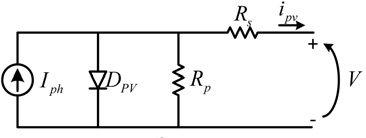
\includegraphics[width=0.6\linewidth]{pv_model}
		\caption{Circuito Equivalente de uma Célula Fotovoltaica \cite{PV-Teory}}
		\label{fig:model_PV}
	\end{center}
\end{figure}

A partir das equações ~\ref{IPV_},~\ref{IPH_},~\ref{IR_} e ~\ref{IRR_} é possível inferir a existência das relações entre a corrente de saída do painel fotovoltaico, sua temperatura e a irradiação solar. De fato, quanto maior a temperatura da célula, menor sua tensão de circuito aberto e, portanto, mais rápida sua variação de corrente. Já em relação à irradiação solar, quanto menor a magnitude desta, menor a corrente máxima da célula, relação clara ao analisar a equação~\ref{IPH_}.

Na figura~\ref{fig:iv_pv_} são apresentadas curvas I-V para diferentes valores de irradiação solar e temperatura de painel, para servirem de demonstração da influência dessas variáveis no comportamento do painel.

\begin{figure}[htbp]%
	\captionsetup{justification=centering}
	\centering
	\subfloat[]{{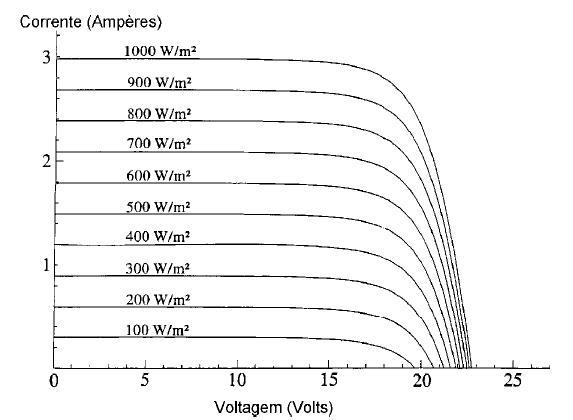
\includegraphics[width=0.45 \linewidth]{iv_PV} }}%
	\qquad
	\subfloat[]{{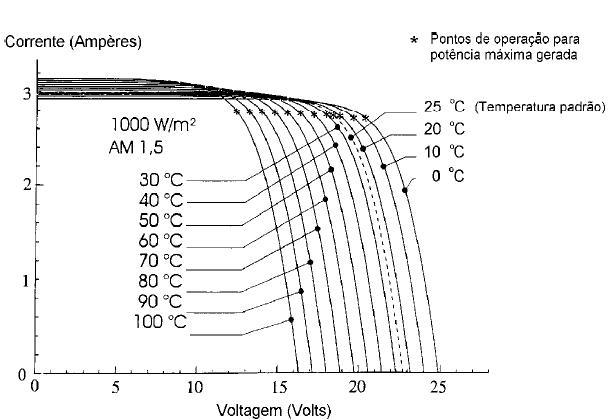
\includegraphics[width=0.45 \linewidth]{iv_pv2} }}%
	\caption{Curvas IxV de painel fotovoltaico para diferentes (a) irradiâncias e (b) temperaturas}%
	\label{fig:iv_pv_}%
\end{figure}


\section{Conversores Estáticos CC/CC}

\subsection{Conversor Ćuk Convencional}

Um conversor Ćuk é um conversor CC-CC baseado na transferência de energia capacitiva que é capaz de fornecer tensão maior ou menor que sua tensão de entrada, com polaridade invertida. Seu circuito pode ser visto na figura~\ref{fig:conv_cuk_circuit}. 

\begin{figure}[htbp]
	\centering
		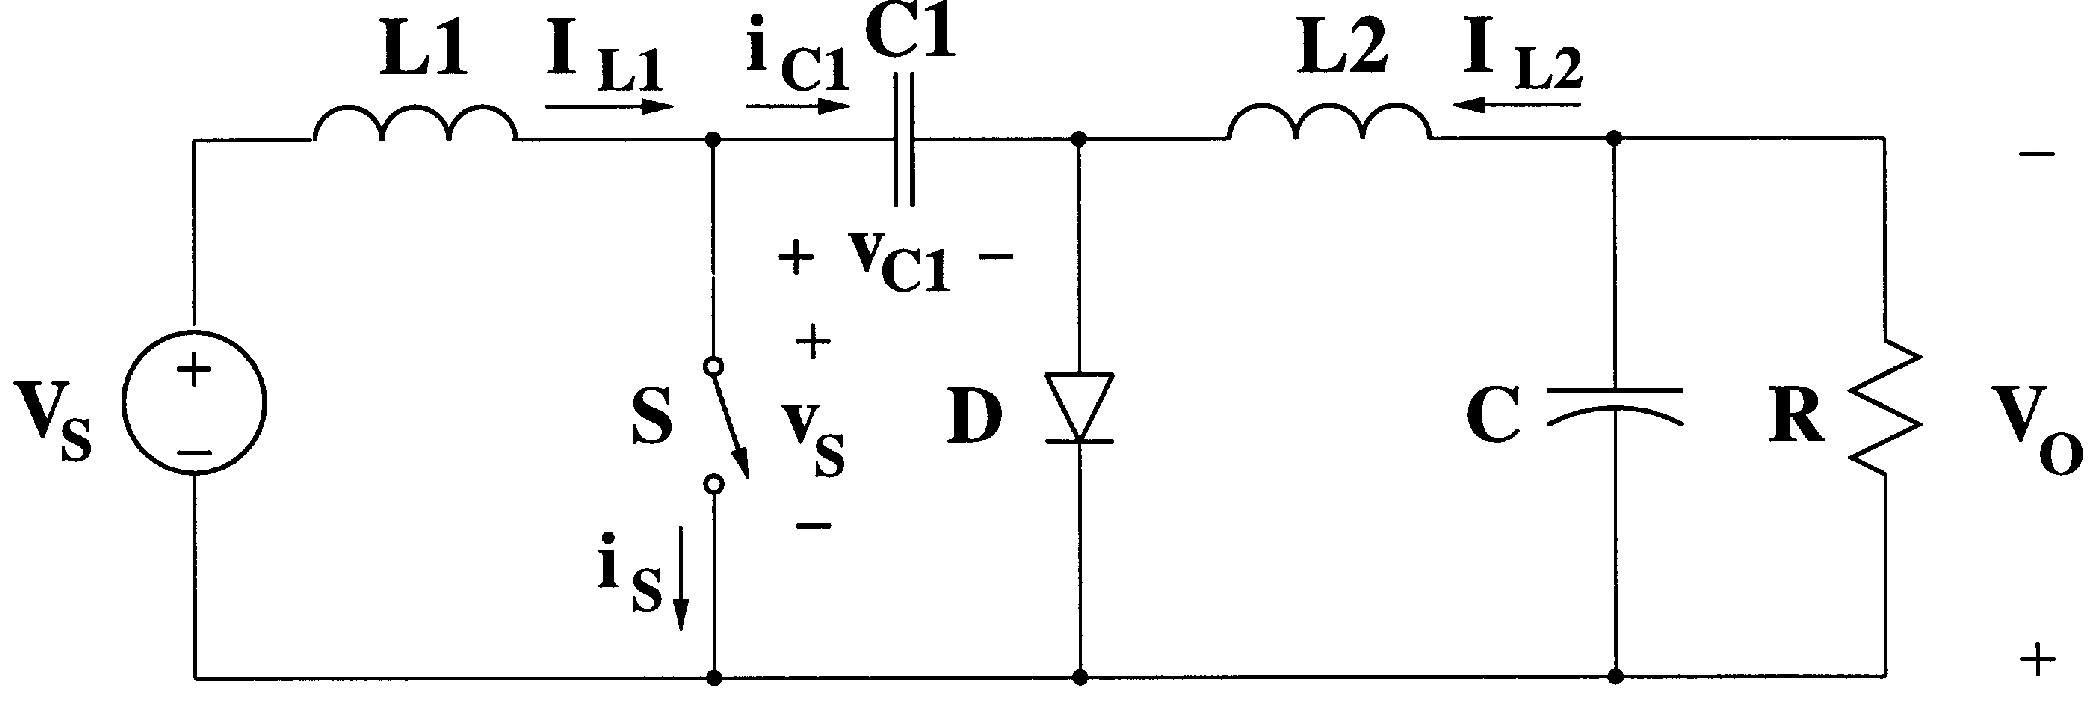
\includegraphics[width=0.55 \linewidth]{conv_cuk_circuit}
		\caption{Conversor Ćuk convencional \cite{RASHID_CUK}}
		\label{fig:conv_cuk_circuit}
\end{figure}

% \begin{figure}[htbp]
% 	\centering
% 		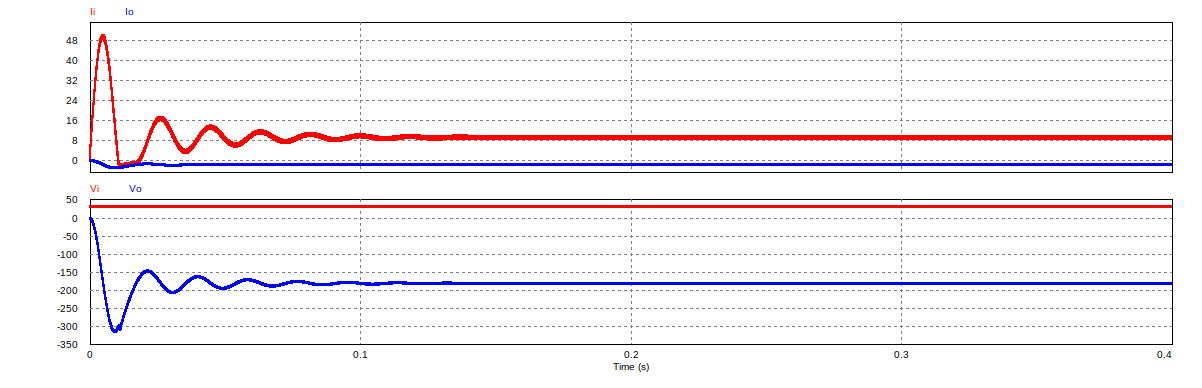
\includegraphics[width= \linewidth]{cuk_conv_In_Out}
% 		\caption{Sinais de entrada  e saída do conversor cuk convencional}
% 		\label{fig:conv_cuk_In_Out}
% \end{figure}

Quando a chave $S$ está fechada (\textit{ON}), os indutores $L1$ e $L2$ são carregados pela tensão de entrada e capacitor $C1$, respectivamente. O capacitor $C1$ polariza inversamente o diodo $D$ e descarrega fornecendo energia para a carga $R$, o capacitor de filtro $C$ e o indutor de filtro $L2$.
Com o transistor representado pela chave $S$ em estado aberto(\textit{OFF}), o indutor de entrada $L1$ carrega o capacitor de transferência de energia $C1$. O diodo $D$ conduz as correntes de ambos $L1$ e $L2$ e, portanto, o indutor $L2$ descarrega fornecendo energia à carga \cite{RASHID_CUK} \cite{JOSEPH_2015_Intervealed_CUK}. 

\begin{figure}[H]
	\captionsetup{justification=centering}
	\centering
		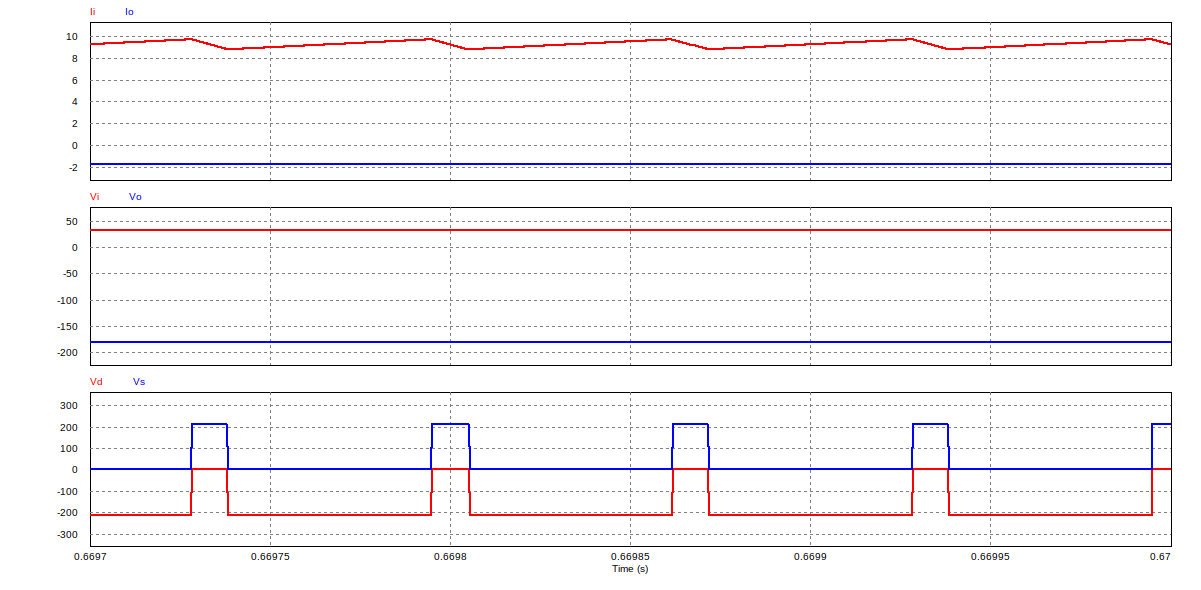
\includegraphics[width= \linewidth]{conv_cuk_signal_details}
		\caption{Sinais de entrada, saída e tensões no transistor e no diodo do conversor cuk convencional}
		\label{fig:conv_cuk_In_Out}
\end{figure}

\begin{figure}[H]
	\captionsetup{justification=centering}
	\centering
		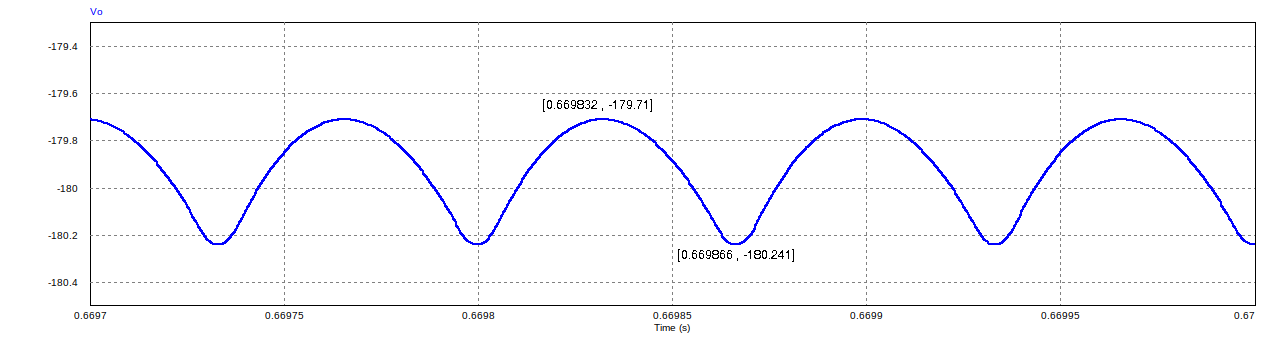
\includegraphics[width= \linewidth]{conv_cuk_Vo_det}
		\caption{Tensão de ripple de saída do conversor cuk convencional}
		\label{fig:conv_cuk_Vo_det}
\end{figure}

A função de transferência CC desse conversor é dada pela equação~\ref{eq:trans_func_cuk_conv}, na qual $d$ é o ciclo de trabalho (\textit{duty cycle}), $V_s$ a tensão de entrada e $V_o$ a tensão de saída \cite{RASHID_CUK} \cite{JOSEPH_2018_Intervelead_cuk}.
\begin{equation}
	M_v = \frac{V_o}{V_s}= - \frac{d}{1-d}
	\label{eq:trans_func_cuk_conv}
\end{equation}
O conversor Ćuk opera em modo de condução contínua para $L1$ > $L_{b1}$ e $L2$ > $L_{b2}$ pelas equações~\ref{eq:cuk_conv_CCM_limits_l1} e ~\ref{eq:cuk_conv_CCM_limits_l2}.

O capacitor de filtro $C$ mínimo para uma certa tensão de ripple $V_r$ pode ser encontrado utilizando a equação~\ref{eq:rip_filt_conv_cuk}. Já a tensão de ripple no capacitor $C1$ pode ser estimada pela equação~\ref{eq:conv_cuk_rip_c1}.
\begin{IEEEeqnarray}{c}%
	L_{b1} = \frac{(1-d)R}{2df} \label{eq:cuk_conv_CCM_limits_l1}\\
	L_{b2} = \frac{(1-d)R}{2f} \label{eq:cuk_conv_CCM_limits_l2} \\
	C_{min} = \frac{(1-d) V_o}{8 V_r L_2 f^2} \label{eq:rip_filt_conv_cuk}\\
	V_{r_{C1}} = \frac{dV_o}{C_1 R f} \label{eq:conv_cuk_rip_c1}
\end{IEEEeqnarray}

Nas equações~\ref{eq:cuk_conv_CCM_limits_l1} a \ref{eq:rip_filt_conv_cuk} $f$ é a frequência de chaveamento do transistor $S$. A figura~\ref{fig:conv_cuk_In_Out} demonstra os sinais de tensão e corrente de entrada e saída do conversor, em estado estacionário, além da tensão no transistor e no diodo do circuito. Já a figura~\ref{fig:conv_cuk_Vo_det} demonstra a tensão de ripple na saída do conversor.

% Vale notar que a função de transferência da equação~\ref{eq:trans_func_cuk_conv} é igual à de um conversor \textit{Buck-Boost}.

% APRESENTA MODELO, PRINCIPIOS E INTRO AO PROJETO
\subsection{Conversor Ćuk Entrelaçado}

Um conversor cuk entrelaçado consiste de  dois conversores cuk convencionais que operam com pulsos defasados nos transistores. A conexão é feita através indutores de saída, que são conectados junto ao capacitor de saída, comum entre todas as fases. A figura~\ref{fig:interv_cuk_conv} apresenta o circuito de um conversor cuk entrelaçado de duas fases. O objetivo principal dessa implementação reduzir o ripple de tensão na saída.

Segundo \citeonline{JOSEPH_2015_Intervealed_CUK}, essa topologia tem o intuito de reduzir o ripple de corrente na entrada e reduzir o stress de chaveamento, sem sacrificar sua eficiência. Para tal, os transistores são ligados um por vez, por um período de ${T_{on}}/{2}$, e somente após passado um período ${T_{off}}/{2}$ do desligamento do transistor anterior. Isso é feito  utilizando-se a técnica de modulação por largura de pulso com deslocamento de fase, \emph{PSPWM}, do inglês \textit{Phase-Shifted Pulse Width Modulation}.

O funcionamento do conversor cuk entrelaçado de duas fases pode ser descrito em 3 modos~\cite{JOSEPH_2015_Intervealed_CUK}:
\begin{itemize}%
	\item Modo 1 ($t_0$-$t_1$): $S_1$ ligado e $S_2$ desligado;
	\item Modo 2 ($t_1$-$t_2$ e $t_3$-$t_4$): $S_1$ e $S_2$ desligados;
	\item Modo 3 ($t_2$-$t_3$): $S_1$ desligado e $S_2$ ligado.
\end{itemize}

No modo 1, ocorre a carga do indutor $L_{1a}$ e a descarga do indutor $L_{1b}$, que fornece energia ao capacitor $C_2$. Enquanto isso, o capacitor $C_1$ para a carga.

Assumindo uma variação linear na corrente dos indutores, a corrente de ripple para os indutores nesse modo pode ser calculada com as equações~\ref{eq:rip_interv_1} a \ref{eq:rip_interv_3}, nas quais $t_1$ é o tempo em que o transistor $S_1$ está ligado, $V_d$ a tensão de entrada e $V_{C_1}$ e $V_{C_2}$ a tensão nos capacitores $C_1$ e $C_2$, respectivamente.
\begin{IEEEeqnarray}{c}
	\Delta I_{L_{1a}} = \frac{t_1 V_d}{L_{1a}} \label{eq:rip_interv_1} \\
	\Delta I_{L_{1b}} = \frac{t_1 \left(V_{C_2} - V_d \right)}{L_{1b}} \label{eq:rip_interv_2} \\
	\Delta I_{L_2} = \frac{t_1 \left( V_{C_1} + V_o\right)}{L_2} \label{eq:rip_interv_3}
\end{IEEEeqnarray}

\begin{figure}[htbp]
	\begin{center}
		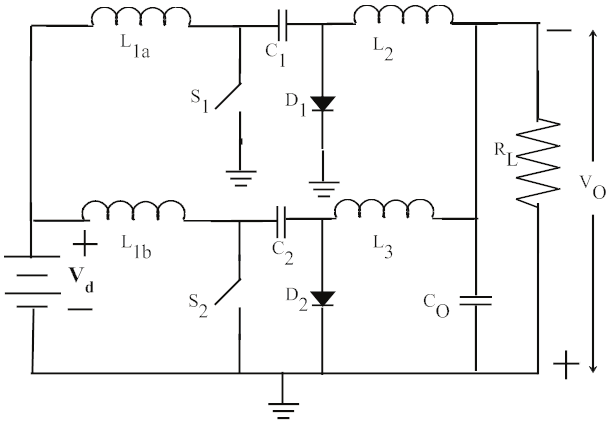
\includegraphics[width=0.55 \linewidth]{interv_cuk_circuit}
		\caption{Conversor Ćuk entrelaçado de duas fases \cite{JOSEPH_2015_Intervealed_CUK}}
		\label{fig:interv_cuk_conv} 
	\end{center}
\end{figure}

% \begin{figure}[htbp]
% 	\begin{center}
% 		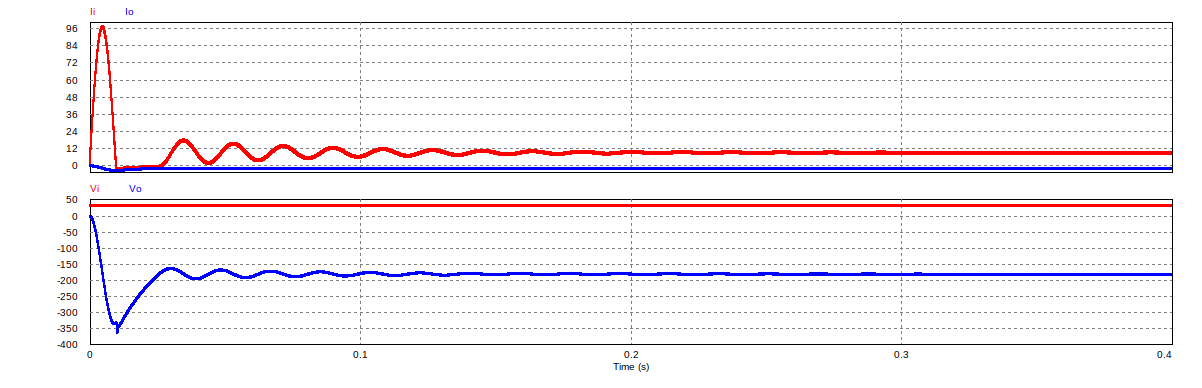
\includegraphics[width= \linewidth]{cuk_interv_In_Out}
% 		\caption{Sinais de entrada e saída do conversor cuk entrelaçado de duas fases}
% 		\label{fig:interv_cuk_In_Out} 
% 	\end{center}
% \end{figure}

\begin{figure}[htbp]
	\captionsetup{justification=centering}
	\centering
		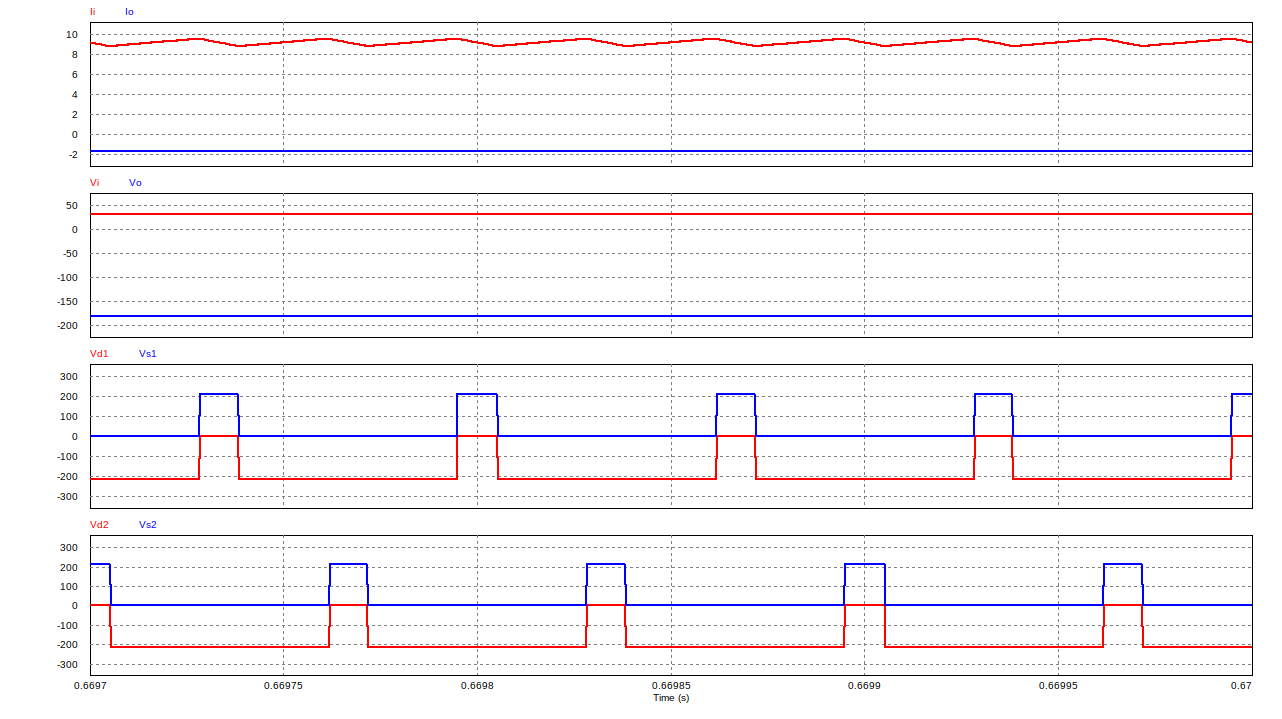
\includegraphics[width= \linewidth]{interv_cuk_signal_details}
		\caption{Sinais de entrada, saída e tensões no transistor e no diodo do conversor cuk entrelaçado de duas fases}
		\label{fig:interv_cuk_In_Out} 
\end{figure}

\begin{figure}[H]
	\captionsetup{justification=centering}
	\centering
		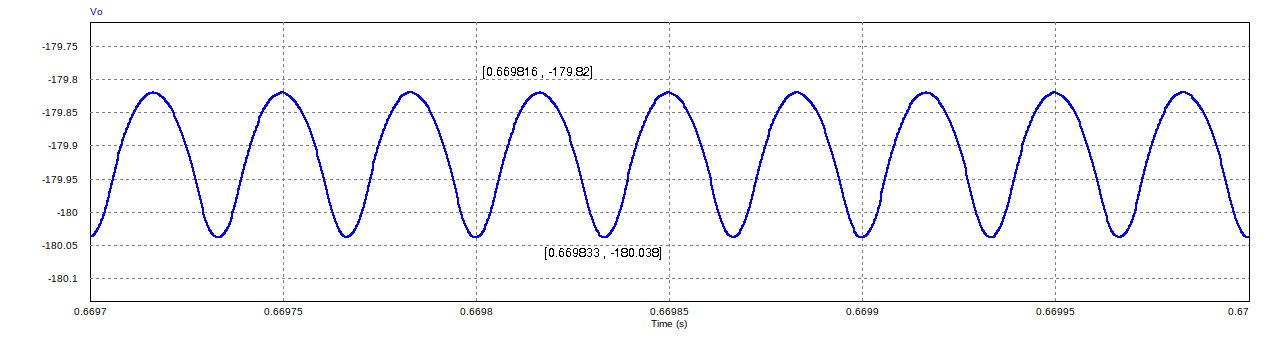
\includegraphics[width= \linewidth]{interv_cuk_Vo_det}
		\caption{Tensão de ripple de saída do conversor cuk entrelaçado de duas fases}
		\label{fig:interv_cuk_Vo_det}
\end{figure}

Quando ambos os transistores estão desligados, ou seja, no modo 2, os indutores de entrada $L_{1a}$ e $L_{1b}$ são descarregados, fornecendo energia aos capacitores $C_1$ e $C_2$, respectivamente, de forma que, entre $t_1$ e $t_2$, $C_1$ carrega a energia que foi fornecida à carga no modo anterior, enquanto que entre $t_3$ e $t_4$, $C_2$ o faz. Além disso, os indutores $L_2$ e $L_3$ fornecem energia à carga e, portanto são descarregados.

Os ripples de corrente para os indutores nesse modo são encontrados utilizando as equações~\ref{eq:rip_interv_4} a \ref{eq:rip_interv_6}
\begin{IEEEeqnarray}{c}
	\Delta I_{L_{1a}} = \frac{t_2 \left(V_{C_1} - V_d\right)}{L_{1a}} \label{eq:rip_interv_4} \\
	\Delta I_{L_{1b}} = \frac{t_2 \left(V_{C_2} - V_d \right)}{L_{1b}}\label{eq:rip_interv_5} \\
	\Delta I_{L_2} = - \frac{t_2 V_o}{L_2} \label{eq:rip_interv_6}
\end{IEEEeqnarray}

No terceiro modo, com $S_2$ ligado, enquanto o indutor $L_{1b}$ continua sendo carregado, o indutor $L_{1a}$ é descarregado, fornecendo energia ao capacitor $C_1$. Por sua vez, o capacitor $C_2$ fornece energia à carga e aos componentes $L_3$, $C_o$.

Através das equações~\ref{eq:rip_interv_1}, \ref{eq:rip_interv_4},\ref{eq:rip_interv_3} e \ref{eq:rip_interv_6}, tem-se a equação da tensão de saída (\ref{eq:vo_interv}), onde $d = T_{on}/T$.
\begin{equation}
 V_o = - \frac{d \cdot V_d}{1 - d} \label{eq:vo_interv}
\end{equation}

Na figura~\ref{fig:interv_cuk_In_Out} são apresentadas as formas de onda dos sinais de entrada e saída do conversor cuk entrelaçado, além das tensões sobre os transistores e diodos de cada uma das fases, através dos quais é possível perceber o defasamento no comando das chaves. Já a figura~\ref{fig:interv_cuk_Vo_det} demonstra a tensão de ripple obtida pela simulação dessa implementação, que equivale a 41\% do valor obtido para a simulação do conversor cuk convencional (figura~\ref{fig:conv_cuk_Vo_det}).

\section{Conversores CC/CA - Inversores tipo fonte de tensão (\textit{VSI})}

% A configuração básica de um inversor tipo fonte de tensão,\textit{VSI}, do inglês \textit{Voltage Source Inverter} é apresentada na figura~\ref{fig:vsi_3fas}. Para a obtenção de um inversor monofásico, em ponte completa, a única alteração necessária é remover um dos braços do circuito trifásico, como pode ser visto na figura~\ref{fig:vsi_1fas}.

% Havendo tensão na entrada do inversor, quando um transistor das semipontes superior ou inferior, nunca ao mesmo tempo, estiver em condução, a tensão CC aparecerá entre um par de condutores na saída alternada\cite{Pomilio_Cap_5}.

% \begin{figure}[h]
% 	\begin{center}
% 		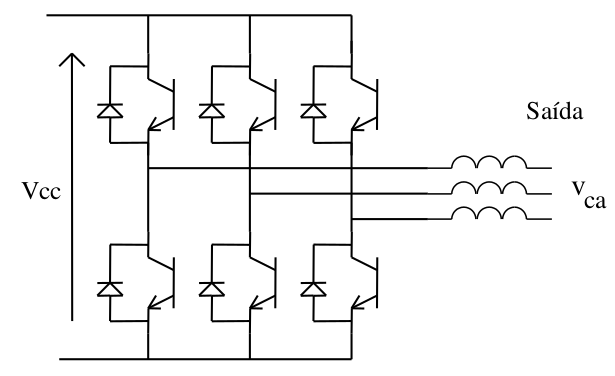
\includegraphics[width=0.55 \linewidth]{vsi_3fas}
% 		\caption{Inversor VSI trifásico \cite{Pomilio_Cap_5}}
% 		\label{fig:vsi_3fas}
% 	\end{center}
% \end{figure}

O inversor de tensão é responsável por converter uma tensão contínua em outra alternada, com frequência e amplitude bem definidas. A topologia de um inversor tipo fonte de tensão, \emph{VSI}, do inglês \textit{Voltage Source Inverter} monofásico em ponte completa pode ser vista na figura~\ref{fig:vsi_1fas}. 

É facilmente perceptível que, caso ambos um transistores de uma das pernas do circuito estejam em condução simultaneamente haverá um curto-circuito na tensão de entrada $v_i$, que corresponde á tensão de barramento CC que alimenta o circuito. Dessa forma deve-se sempre garantir que apenas um dos transistores em cada perna conduza em um certo período de tempo.

No total o circuito apresenta cinco possíveis estados de operação, sendo quatro com tensão de saída definida(estados 1 a 4) e um com tensão indefinida(estado 5). O estados e sua tensão de saída correspondente são \cite{RASHID_VSI}:

\begin{table}[h]%
	\centering
	\begin{tabular}{|c|c|c|c|c|c|}
	\hline
	\rowcolor[HTML]{C0C0C0} 
	\textbf{Estado} & \textbf{$S_{1_+}$} & \textbf{$S_{1_-}$} & \textbf{$S_{2_+}$} & \textbf{$S_{2_-}$} & \textbf{Tensão de Saída} \\ \hline
	\textit{1}      & Ligado             & Desligado          & Desligado          & Ligado             & $v_i$                    \\ \hline
	\textit{2}      & Desligado          & Ligado             & Ligado             & Desligado          & $-v_i$                   \\ \hline
	\textit{3}      & Ligado             & Desligado          & Ligado             & Desligado          & 0                        \\ \hline
	\textit{4}      & Desligado          & Ligado             & Desligado          & Ligado             & 0                        \\ \hline
	\textit{5}      & Desligado          & Desligado          & Desligado          & Desligado          & $v_i$ ou $-v_i$          \\ \hline
	\end{tabular}
	\caption{Possíveis estados de operação de um VSI em Ponte Completa}
	\label{table:VSI_states}
\end{table}

\begin{figure}[htbp]
	\begin{center}
		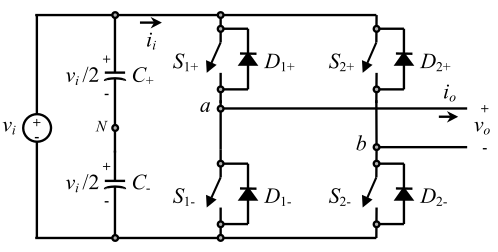
\includegraphics[width=0.65 \linewidth]{vsi_1fas}
		\caption{Inversor VSI monofásico em ponte completa \cite{RASHID_VSI}}
		\label{fig:vsi_1fas}
	\end{center}
\end{figure}

Como um inversor deve ser capaz de fornecer tensão com amplitude \emph{bem definida}, o estado 5 deve ser evitado. Para isso, a modulação utilizada deve garantir que a todo momento um, e apenas um, dos transistores de cada perna esteja conduzindo corrente. Várias técnicas de modulação podem ser aplicadas a inversores VSI de ponte completa, entre elas as de PWM bipolar e unipolar\cite{RASHID_VSI}.

\subsection{Inversor com Modulação por Largura de Pulso Bipolar}

No inversor com PWM bipolar apenas os estados 1 e 2 da tabela~\ref{table:VSI_states} são utilizados para gerar o sinal de saída, de modo que este apresenta apenas dois valores, $v_i$ e $-v_i$.

Deseja-se que a tensão alternada na saída siga uma forma de onda que,para este trabalho é senoidal. A técnica de PWM baseada em sinal de portadora atende a essa questão ao definir os estados dos transistores a partir da comparação entre um sinal que corresponde à saída desejada $v_m$, chamado de modulante, e uma forma de onda triangular $v_p$, chamada de portadora.

Define-se que, enquanto o sinal modulante é maior que a portadora, o estado 1 é acionado, ou seja, os transistores $S_{1_+}$ e $S_{2_-}$ entram em condução, enquanto so transistores $S_{1_-}$ e $S_{2_+}$ são desligados. O estado 2 é acionado quando o sinal de portadora apresenta maior tensão que o sinal modulante. 

O sinal obtido na saída de um inversor que segue esta técnica é, basicamente, uma forma de onda senoidal que apresenta amplitude fundamental $\hat{v}_o$ a qual satisfaz a expressão~\ref{eq:VSI_bip_vo}, onde $m_a$ é o índice de modulação, ou razão de modulação de amplitude, representada pela equação~\ref{eq:mod_ind_bip} \cite{RASHID_VSI}.
% \vspace{-10pt}
\begin{IEEEeqnarray}{c}
	\hat{v}_o = v_{ab} = v_i m_a \label{eq:VSI_bip_vo} \\
	m_a = \frac{\hat{v}_m}{\hat{v}_p} \label{eq:mod_ind_bip}
\end{IEEEeqnarray}
% A equação~\ref{eq:VSI_bip_vo}, porém, só é satisfeita na região linear da modulação, quando $m_a < 1$. Para situações de sobremodulação, em que a amplitude do sinal modulante é maior que o sinal da portadora, é a expressão~\ref{eq:VSI_bip_vo_over} que representa a fundamental $\hat{v}_o$.
% \begin{equation}
% 	v_i < \hat{v}_o = \hat{v_{ab}} < \frac{4}{\pi}v_i \label{eq:VSI_bip_vo}
% \end{equation}
\vspace{-10pt}
\begin{figure}[htbp]%
	\captionsetup{{justification=centering}}
	\centering%
		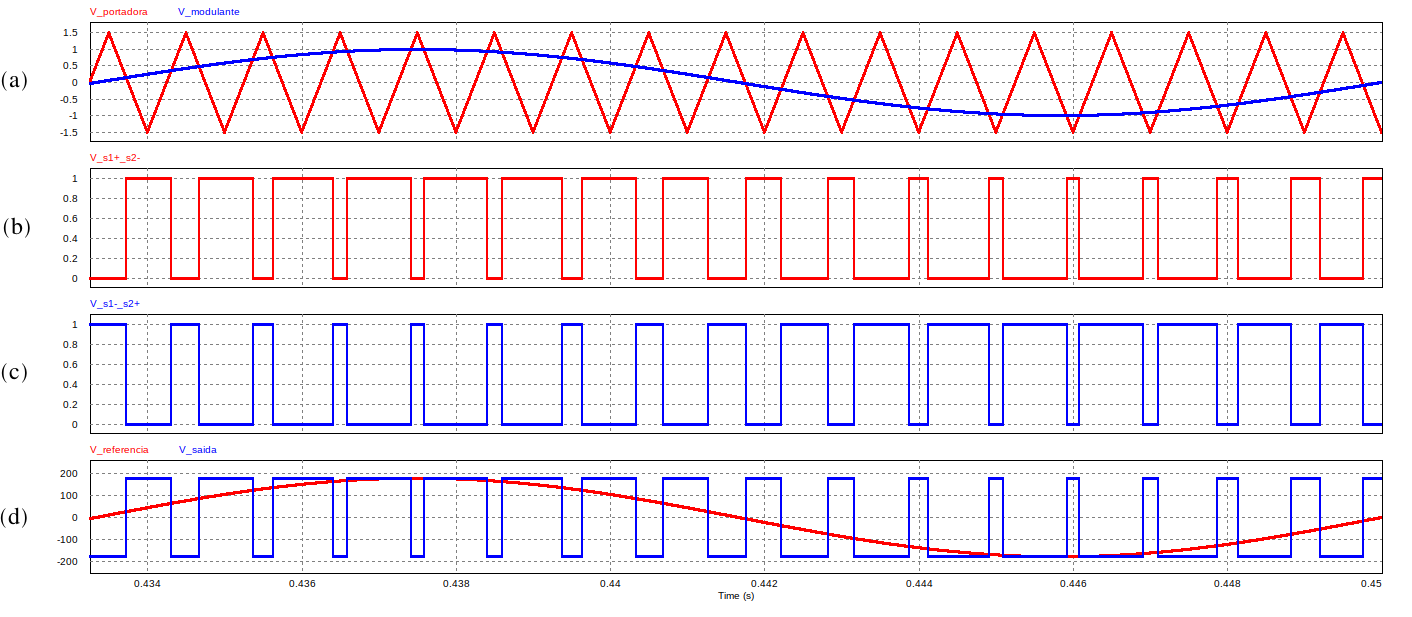
\includegraphics[width= \linewidth]{vsi_bip_func}
		\caption{Formas de onda do inversor VSI com PWM bipolar}
		\label{fig:vsi_bip_func_graph}
\end{figure}

A figura~\ref{fig:fft_vsi_bip} demonstra o conteúdo harmônico da tensão de saída desse inversor para uma frequência de chaveamento de 1kHz. É possível perceber a presença dos harmônicos pares e ímpares dessa frequência, de forma que a distorção harmônica total da tensão de saída é de 186\%, considerando o valor esperado como uma onda senoidal de 60Hz.

\begin{figure}[H]%
	\captionsetup{{justification=centering}}
	\centering%
		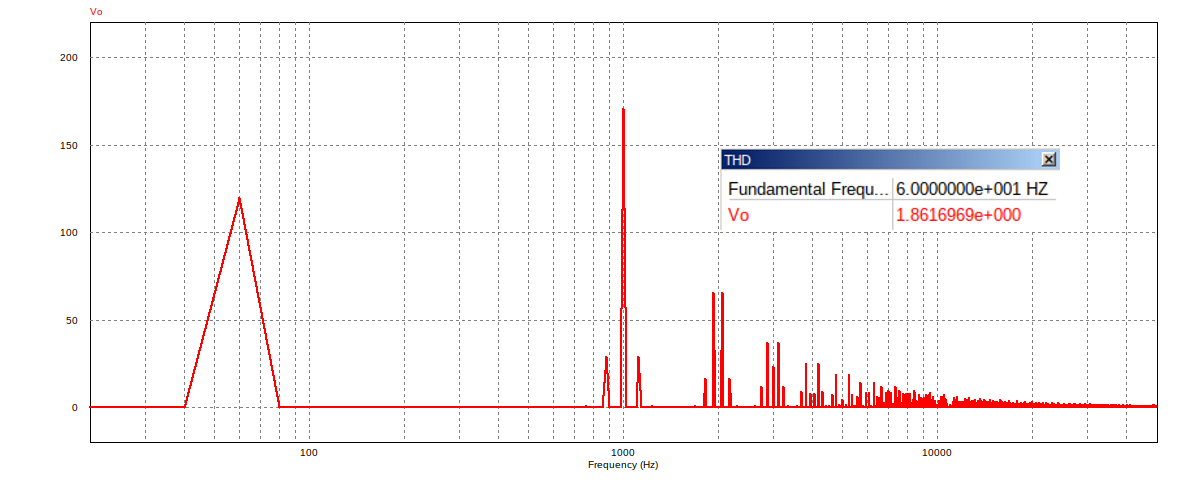
\includegraphics[width= \linewidth]{fft_vsi_bip}
		\caption{Conteúdo harmônico da tensão de saída do inversor VSI Bipolar}
		\label{fig:fft_vsi_bip}
\end{figure}

\subsection{Inversor com Modulação por Largura de Pulso Unipolar}

Já em um inversor com PWM unipolar apenas os estados 1, 2, 3 e 4 da tabela~\ref{table:VSI_states} são utilizados para gerar o sinal de saída. Dessa forma a tensão alternada obtida apresenta três possíveis valores: $0$, $v_i$ e $-v_i$.

Neste tipo de modulação são utilizados dois sinais modulantes $v_m$ e $-v_m$. Cada modulante é responsável pela tensão em um dos braços do inversor, em relação ao ponto neutro ($N$), de modo que $v_m$ controla a tensão $v_{aN}$ e $-v_{m}$ é responsável por $v_{bN}$. A amplitude da tensão de saída para este método é expressa pela equação~\ref{eq:VSI_uni_vo}, encontrada pela combinação das equações~\ref{eq:VSI_uni_1} e \ref{eq:VSI_uni_1}.
\begin{IEEEeqnarray}{c}%
	v_{bN} = -v_{aN} \label{eq:VSI_uni_1} \\
	v_o = v_{aN} - v_{bN} \label{eq:VSI_uni_2}\\
	\hat{v}_o = 2 \cdot \hat{v}_{aN} = v_i m_a \label{eq:VSI_uni_vo}
\end{IEEEeqnarray}
Segundo \citeonline{RASHID_VSI}, devido ás tensões de fase ($V_{aN}$ e $v_{bN}$) serem idênticas e defasadas de 180º, a tensão de saída não apresenta harmônicos pares, presentes em inversores que utilizam o método de modulação bipolar. 

Essa característica permite que inversores que utilizam a modulação unipolar utilizem filtros menores para obter tensão e corrente de alta qualidade, utilizando a mesma frequência de chaveamento que inversores com modulação bipolar\cite{RASHID_VSI}.

\begin{figure}[htbp]%
	\captionsetup{{justification=centering}}
	\centering%
		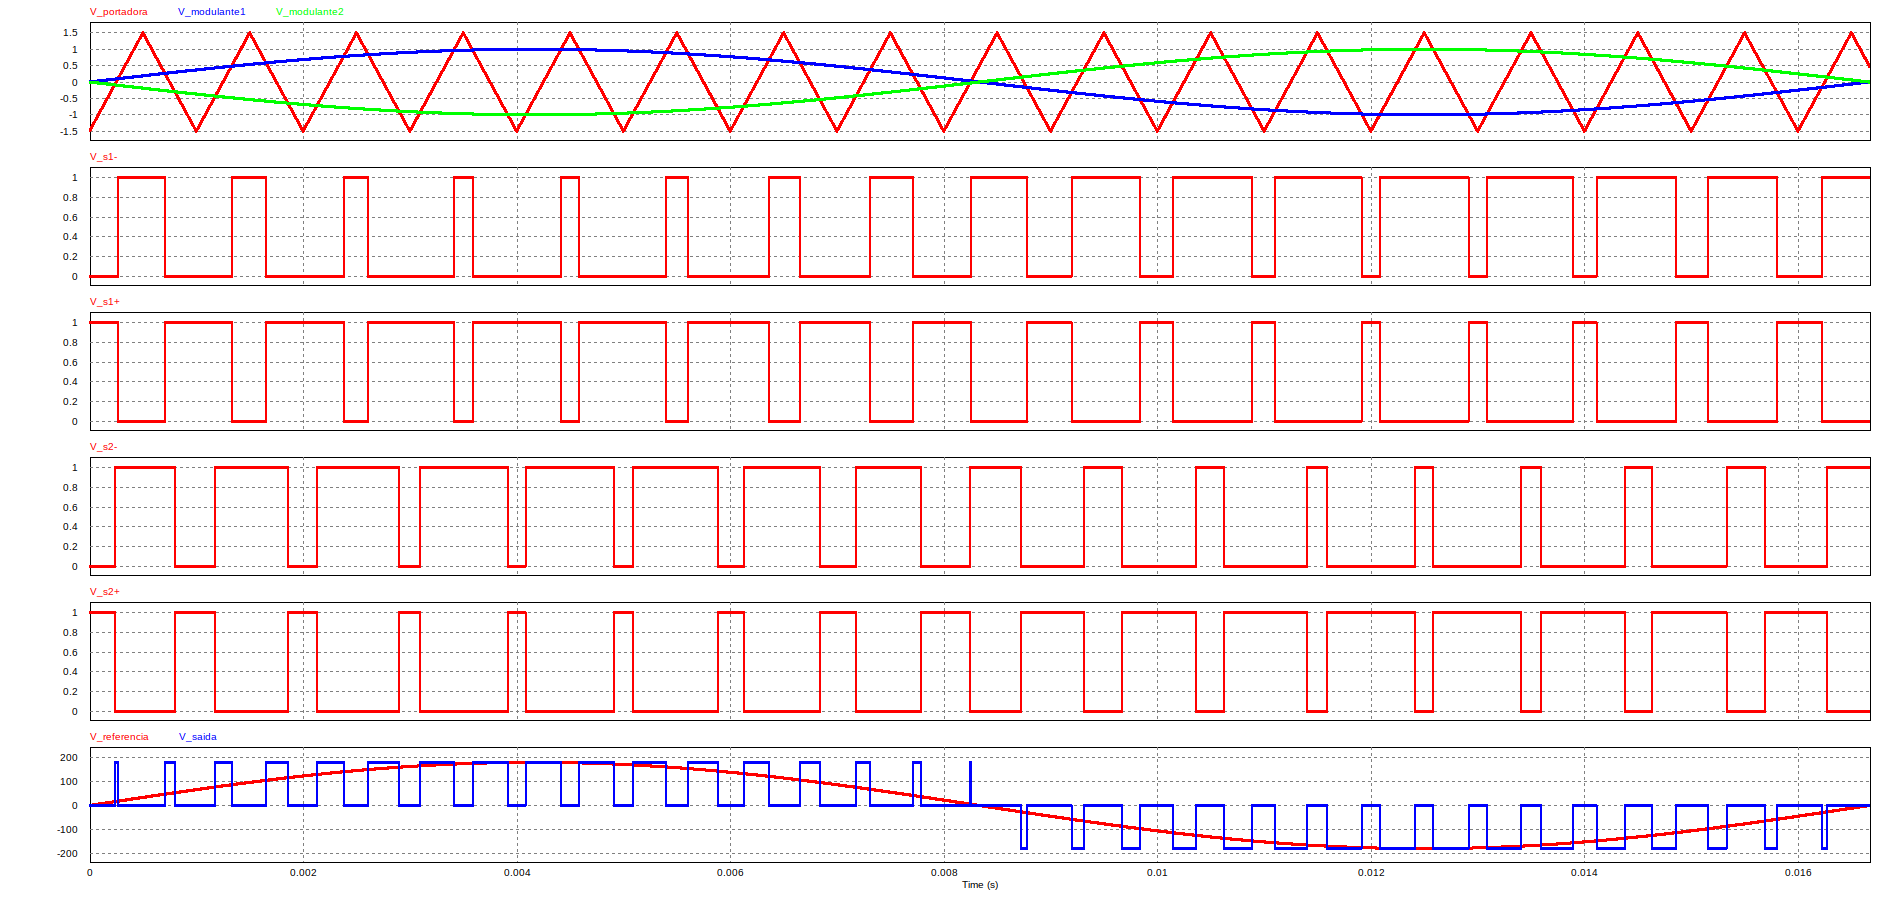
\includegraphics[width= \linewidth]{vsi_uni_func}
		\caption{Formas de onda do inversor VSI com PWM unipolar}
		\label{fig:vsi_uni_func_graph}
\end{figure}

A figura~\ref{fig:fft_vsi_unip} demonstra o conteúdo harmônico da tensão de saída desse inversor para uma frequência de chaveamento de 1kHz. É possível perceber a presença apenas dos harmônicos pares dessa frequência, de forma que a distorção harmônica total da tensão de saída é de 95\%, considerando o valor esperado como uma onda senoidal de 60Hz. 

Quando comparada ao valor encontrado para o inversor VSI bipolar, apresentado na figura~\ref{fig:fft_vsi_bip}, a distorção harmônica apresentada para o inversor com controle unipolar equivale a, aproximadamente, metade da distorção harmônica obtida pelo inversor anterior. 

\begin{figure}[H]%
	\captionsetup{{justification=centering}}
	\centering%
		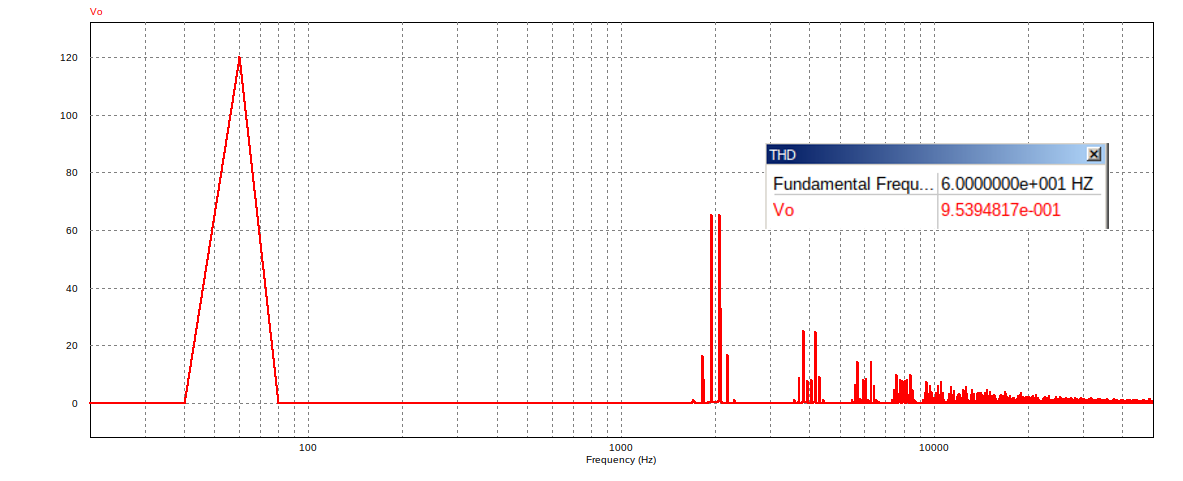
\includegraphics[width= \linewidth]{fft_vsi_uni}
		\caption{Conteúdo harmônico da tensão de saída do inversor VSI Unipolar}
		\label{fig:fft_vsi_unip}
\end{figure}

\section{Inversor Integrado (CC/CA)}
\subsection{Inversor Ćuk Integrado}

A integração de estágios consiste na união dos estágios subidor de tensão(CC-CA) e inversor (CC-CA) em um único estágio CC-CA, com o circuito mais simples e com menor número componentes. 

Segundo proposto por \citeonline{LUIGI_int_top}, a primeira simplificação do conversor cuk integrado ao inversor de tensão em ponte completa é a retirada do capacitor e do indutor de filtro na saída no estágio elevador de tensão, ou seja, no barramento CC. Dessa forma, tensão e corrente do primeiro estágio são entregues diretamente ao inversor. A segunda, e última simplificação possível nessa integração é a retirada do diodo do conversor cuk, uma vez que os diodos anti-paralelos do inversor são capazes de efetuar sua função.

Na figura~\ref{fig:integ_cuk_circ} é possível ver o circuito final resultante das simplificações descritas, no qual os componentes $L_b$, $S_b$ e $C_b$ advém de um conversor cuk convencional. 

% Para conexão com a rede elétrica, como fonte de corrente, o capacitor de saída $C_o$ da figura~\ref{fig:integ_cuk_circ} pode ser simplesmente substituído pela rede\cite{LUIGI_int_top}. 

\begin{figure}[H]
	\begin{center}
		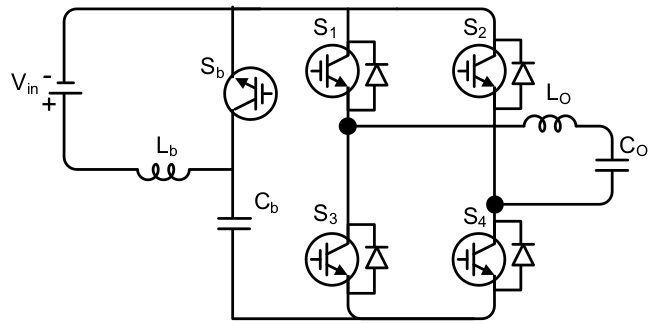
\includegraphics[width=0.65 \linewidth]{integ_cuk_circ}
		\caption{Inversor Ćuk Integrado \cite{LUIGI_int_top}}
		\label{fig:integ_cuk_circ}
	\end{center}
\end{figure}

% \begin{figure}[H]
% 	\begin{center}
% 		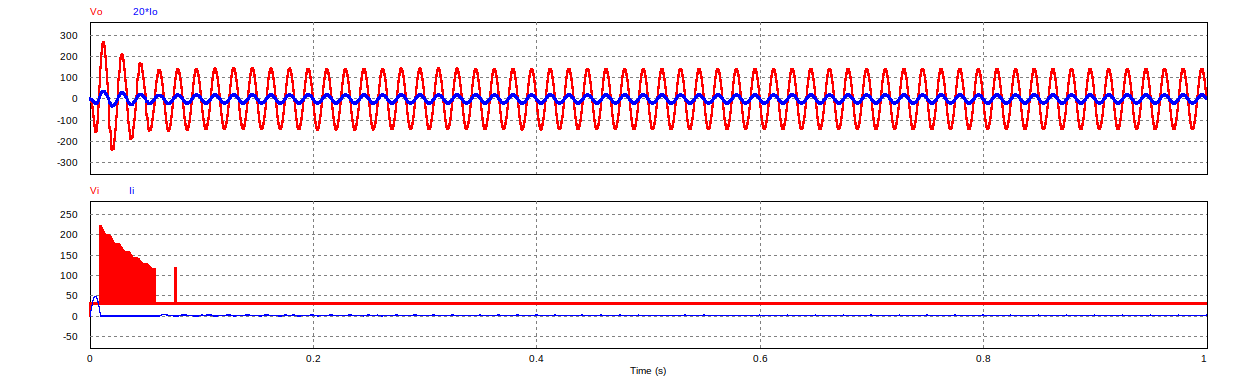
\includegraphics[width=\linewidth]{cuk_integ_In_Out}
% 		\caption{Sinais de entrada e saída do inversor cuk integrado}
% 		\label{fig:integ_cuk_In_Out}
% 	\end{center}
% \end{figure}

A figura~\ref{fig:integ_cuk_In_Out_zoom} apresenta os sinais e entrada e saída para um inversor cuk integrado com controle PWM unipolar, com filtro de saída indutivo. É possível perceber que a tensão de entrada é constante enquanto a corrente varia com frequência de aproximadamente duas vezes a frequência da saída.

\begin{figure}[htb]
	\centering
		\captionsetup{{justification=centering}}
		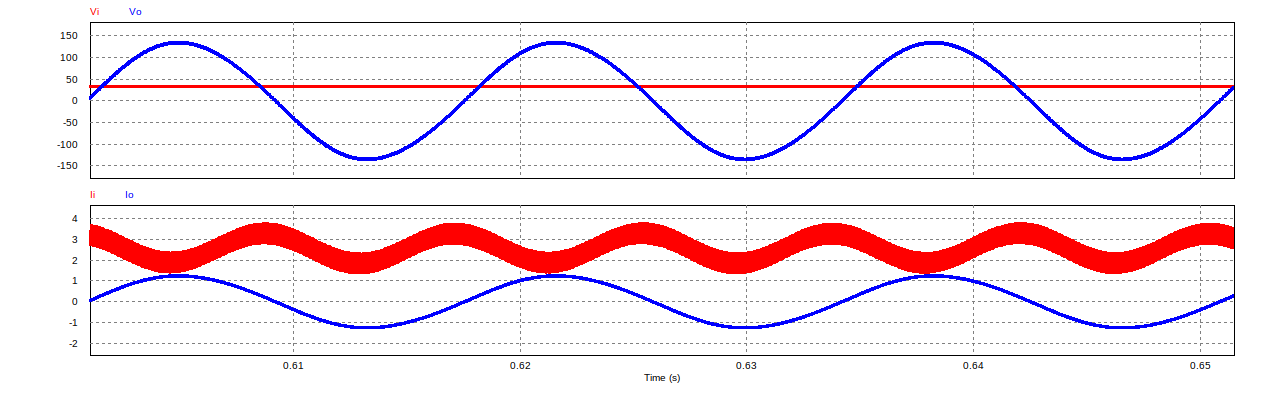
\includegraphics[width= \linewidth]{cuk_integ_In_Out_zoom_2}
		\caption{Sinais de entrada e saída do inversor cuk integrado em regime permanente}
		\label{fig:integ_cuk_In_Out_zoom}
\end{figure}


\section{Rastreador de ponto de máxima potência (\textit{MPPT})}

O ponto de máxima potência de sistema de geração solar dependem da irradiação solar e da temperatura das células geradoras e, portanto, o rastreamento deste ponto de operação deve ser feito de forma constante. Para esse controle é geralmente utilizado um rastreador de ponto de máxima potência, \emph{MPPT}, do inglês \textit{Maximum Power Point Tracker} \cite{Talha_MPPT}. 

Este dispositivo monitora tensão e corrente fornecidas pelo painel fotovoltaico para determinar o ponto de operação no qual este fornecerá a máxima potência disponível, de modo a aumentar, desta forma, a eficiência do painel. Existem vários algoritmos de controle do ponto de máxima potência, e a seguir serão tratados dois, o método P\&O (perturba e observa) e o método da condutância incremental (IC). Estes métodos são amplamente utilizados devido, principalmente, a facilidade de implementação \cite{MPPT_P&O_IC}\cite{Talha_MPPT}.

A figura~\ref{fig:mppt_power_demo} demonstra a irradiância (S), a potência fornecida pelo painel e a potência de saída de um conversor cuk convencional com a utilização de um MPPT utilizando o método de perturba e observa. O possível perceber a acomodação do sistema para obter sempre a máxima potência disponível no painel.   

\subsection{Método Perturba e Observa (P\&O)}

Neste método, é inserida na tensão de operação do painel fotovoltaico uma pequena perturbação, que pode ser positiva ou negativa, de acordo com a necessidade. Caso após a perturbação a potência fornecida aumenta, então é aplicada outra perturbação no mesmo sentido da anterior. Quando a potência reduz após a alteração da tensão a perturbação é invertida. Esse processo é repetido periodicamente até encontrar o ponto de operação desejado\cite{Talha_MPPT}.

A constante perturbação da tensão faz com que a potência fornecida pelo painel varie. Desta forma o ponto de máxima potência nunca é completamente atingido, já que o sistema fica oscilando em torno deste. Para reduzir a influência dessa oscilação, a amplitude da perturbação é mantida sempre baixa \cite{MPPT_P&O_IC}.

Como já dito, uma das vantagens deste método de MPPT está na simplicidade de sua implementação mas, além disso, apresenta alta eficiência para irradiância solar alta e constante. Já entre as desvantagens estão a possibilidade de falha para variações abruptas de irradiância e o fato de o ponto de máxima potência não ser devidamente atingido, principalmente\cite{MPPT_P&O_IC}.

Um fluxograma que representa o funcionamento do algoritmo P\&O pode ser visto na figura~\ref{fig:PeO_Flux}.

\begin{figure}[H]
	\begin{center}
		\includegraphics[width=0.65 \linewidth]{p_and_o_flowchart}
		\caption{Fluxograma do Método P\&O, baseado no diagrama de \citeonline{Talha_MPPT}}
		\label{fig:PeO_Flux}
	\end{center}
\end{figure}

\subsection{Método de Condutância Incremental (IC)}

Este método se baseia no princípio de que a inclinação da potência, em relação à tensão é zero no ponto de máxima potência, positiva à esquerda e negativa à direita deste. Além disso, a perturbação no ciclo de trabalho pode ser parada quando o ponto de máxima potência é encontrado. Enquanto esta condição não é satisfeita a direção da perturbação é definida pela relação entre $\frac{\Delta I}{\Delta V}$ e $\frac{I}{V}$ \cite{Talha_MPPT}\cite{MPPT_P&O_IC}.

Dessa forma, quando a equação~\ref{eq:incCond_mai0} é satisfeita, a perturbação seguinte é positiva e, para a equação~\ref{eq:incCond_men0}, negativa.
\begin{align}%
	\frac{\Delta I}{\Delta V} + \frac{I}{V} &= 0 \qquad \text{No ponto de máxima potência} \label{eq:incCond_at_mpp}\\
	\frac{\Delta I}{\Delta V} + \frac{I}{V} &> 0 \qquad \text{Esquerda do ponto de máxima potência} \label{eq:incCond_mai0}\\
	\frac{\Delta I}{\Delta V} + \frac{I}{V} &< 0 \qquad \text{Direita do ponto de máxima potência} \label{eq:incCond_men0}
\end{align}

Devido a ruído e erros de medição, a situação da equação~\ref{eq:incCond_at_mpp} é raramente satisfeita e, portanto, utiliza-se de uma tolerância $\epsilon$ tal qual, se o módulo da soma descrita na equação~\ref{eq:incCond_at_mpp} for menor que o valor de $\epsilon$, é definido que o ponto de máxima potência foi encontrado e as perturbações são interrompidas\cite{Talha_MPPT}.

A principal vantagem desse método em relação ao P\&O está na maior tolerância a variações rápidas irradiação solar, além do fato de ser capaz de interromper as perturbações após o ponto de operação ter sido definido. Entretanto, o custo e a complexidade do sistema são suas principais desvantagens\cite{MPPT_P&O_IC}.

Um fluxograma que representa o funcionamento do algoritmo de condutância incremental pode ser visto na figura~\ref{fig:IncCond_Flux}.

\begin{figure}[htb]
	\begin{center}
		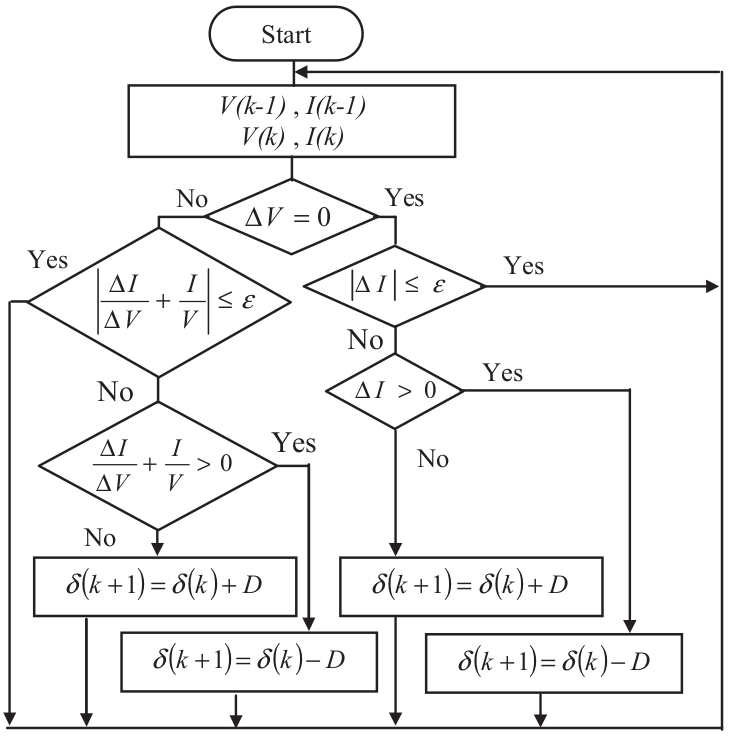
\includegraphics[width=0.6 \linewidth]{incCond_flow}
		\caption{Fluxograma do método de indutância incremental \cite{Talha_MPPT}}
		\label{fig:IncCond_Flux}
	\end{center}
\end{figure}


\begin{figure}[H]
	\captionsetup{justification=centering}
	\centering
		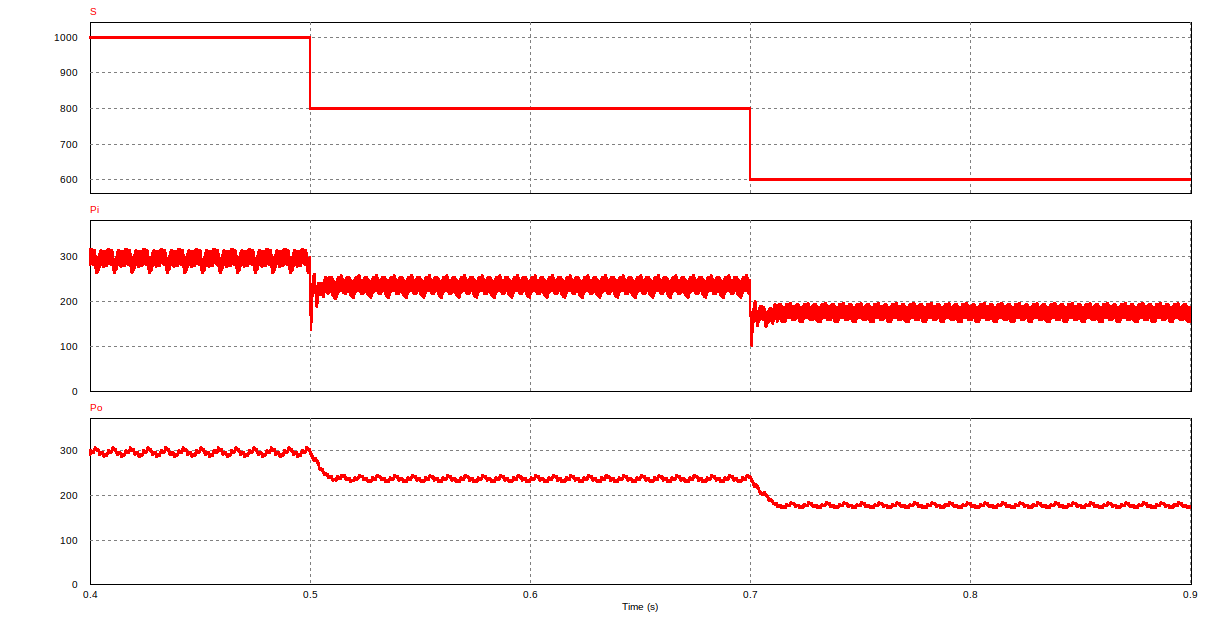
\includegraphics[width= \linewidth]{mppt_power_demo}
		\caption{Potências de entrada e saída de um conversor cuk com MPPT P\&O}
		\label{fig:mppt_power_demo}
\end{figure}

\section{Filtro}

Para conectar o sistema a rede elétrica é necessário filtrar a tensão gerada a fim para reduzir os harmônicos presentes e fazer com que o sinal se assemelhe à uma senoide, e não a um trem de pulsos. Esse processo é feito com a inclusão de um filtro passivo entre o inversor e a rede da concessionária de energia.

Podem ser empregados três diferentes tipos de filtros L, LC e LCL. Destes, o último é mais utilizado atualmente devido a sua maior eficiência e ao fato de minimizar a distorção da corrente injetada na rede elétrica\cite{LCL_FILTER}\cite{LCL_FILTER_Reznik}.

A topologia do filtro LCL pode ser vista na figura~\ref{fig:lcl_filt_top}.

\begin{figure}[htbp]%
	\centering
		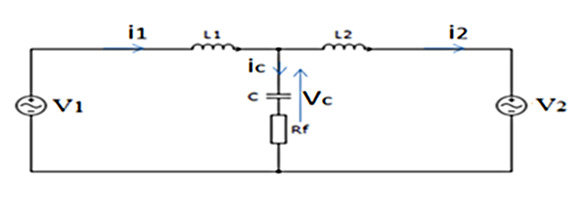
\includegraphics[width=0.7 \linewidth]{lcl_filt_top}
		\caption{Topologia do filtro LCL monofásico\cite{LCL_FILTER}}
		\label{fig:lcl_filt_top}
\end{figure}

Para o projeto do filtro LCL, inicialmente é necessário encontrar os valores de impedância e capacitância base, $Z_b$ e $C_b$, de acordo com as equações~\ref{eq:lcl_zb} e ~\ref{eq:lcl_cb} nas quais $P_n$ é a potência nominal do sistema, $V_g$ a tensão nominal da rede, e $f$ a frequência da rede elétrica.
\begin{IEEEeqnarray}{c}%
	Z_b = \frac{V_g^2}{P_n} \label{eq:lcl_zb}\\
	C_b = \frac{1}{2 \pi f Z_b} \label{eq:lcl_cb}
\end{IEEEeqnarray}

Os indutores $L_1$ e $L_2$ podem ser encontrados a partir das equações~\ref{eq:lcl_l1} e \ref{eq:lcl_l2}, respectivamente. Nessas equações $V_{CC}$ é a tensão do barramento CC ao qual o inversor está conectado, $f_{sw}$ é a frequência de chaveamento do inversor e $\Delta I_{L1_{max}}$ a variação máxima de corrente desejada no indutor, $k_a$ é a atenuação desejada e $C$ o valor do capacitor, definido pela equação~\ref{eq:lcl_c}.
\begin{IEEEeqnarray}{c}%
	L_1 = \frac{V_{CC}}{6 f_{sw} \Delta I_{L1_{max}}} \label{eq:lcl_l1}	\\
	L_2 = \frac{\sqrt{\frac{1}{k_a ^2 }}+1}{\left(2 \pi f_{sw} \right)^2 C} \label{eq:lcl_l2}\\
	C = k C_b \label{eq:lcl_c}
\end{IEEEeqnarray}

A frequência de ressonância do filtro implica diretamente no valor do resistor de ressonância, $R_f$ e pode ser calculada a partir dos valores de $L_1$, $L_2$ e $C$, como demonstra a equação~\ref{eq:lcl_fres}. Além disso, caso essa frequência não satisfaça a equação~\ref{eq:lcl_fres_law}, o filtro deve ser recalculado para outro valor de atenuação.
\begin{IEEEeqnarray}{c}%
	f_{res} = \frac{1}{2 \pi} \sqrt{\frac{L_1+L_2}{L_1 L_2 C}} \label{eq:lcl_fres}\\
	10f_g < f_{res} < 0,5 f_{sw} \label{eq:lcl_fres_law}
\end{IEEEeqnarray}

O resistor $R_f$ é responsável por atenuar parte da oscilação de tensão proveniente do chaveamento, a fim de evitar a ressonância e deve ter o valor equivalente a um terço da impedância do capacitor $C$ na frequência de ressonância\cite{LCL_FILTER_Reznik}, assim como demonstra a equação~\ref{eq:lcl_rf}.

\begin{equation}
	R_f = \frac{1}{6 \pi f_{res} C} \label{eq:lcl_rf}
\end{equation}

% Para que o filtro seja estável, é necessário que a relação definida pela equação~\ref{eq:f_res_eq2}, na qual $f$ é a frequência da rede, $f_{sw}$ a frequência de chaveamento do inversor e $f_{res}$ a frequência de ressonância do filtro, definida na equação~\ref{eq:f_res_eq1}\cite{LCL_FILTER}.
% \begin{IEEEeqnarray}{c}
% 	f_{res} = \frac{1}{2 \pi} \sqrt{\frac{L_1 + L_2}{L_1 L_2 C}} \label{eq:f_res_eq1} \\
% 	10f < f_{res} < 0,5 f_{sw} \label{eq:f_res_eq2}
% \end{IEEEeqnarray}

% O capacitor $C$ é escolhido de modo a otimizar o fator de potência, dessa forma, seu cálculo apresenta um fator, $k$ que representa a porcentagem de energia reativa máxima que o componente pode gerar. A equação~\ref{eq:LCL_C}, na qual $f$ e $V$ são a frequência e a tensão da rede, respectivamente e $P$ a potência nominal do sistema, define o valor máximo do capacitor.
%  \begin{equation}
% 	C_{max} = \frac{Pk}{6 \pi f V^2} \label{eq:LCL_C}
%  \end{equation}

%  Para o cálculo dos indutores $L_1$ e $L_2$ é preciso primeiramente definir a queda de tensão máxima desejada, devido ao filtro. A queda de tensão $\Delta V$ é definida pela equação~\ref{eq:LCL_L},na qual $I$ é a corrente nominal. 
 
%  Além disso, a corrente de ripple no indutor $L_1$ é geralmente escolhida entre $10\%$ e $20\%$, enquanto a da rede não pode ser superior a $3\%$ da corrente nominal\cite{LCL_FILTER}.

%  \begin{IEEEeqnarray}{c}
% 	 \Delta V = 2 \pi f I (L_1 + L_2)\label{eq:LCL_L}\\
% 	 0,1I<\Delta I_{L1}<0,2I \\
% 	 \Delta I_{L2} < 0,03I \label{eq:lcl_deltaI2}
%  \end{IEEEeqnarray}


%  O resistor de amortecimento $R_f$ limita os efeitos de ressonância do filtro e pode ser encontrado de forma empírica.

\chapter{Desenvolvimento do Projeto}  \label{cap:project}

Para o desenvolvimento do projeto, primeiramente é necessário definir a potência a ser utilizada no sistema. Após isso, é escolhido um painel fotovoltaico comercial para que seus parâmetros sejam utilizados no modelo utilizado nas simulações. Com as características do painel é possível projetar os conversores CC/CC e, com estes, os inversores responsáveis pela conversão CC/CA.

Com os inversores funcionais, são projetados os sistemas de rastreamento de máxima potência, responsável por otimizar a potência obtida do painel fotovoltaico e o filtro LCL, que condiciona o sinal de onda quadradas obtido pelos inversores a uma senoide que pode ser conectada à rede elétrica.

Como no projeto estão em estudos microinversores os quais são conectados a um único painel fotovoltaico, foi escolhido um painel de potência média no mercado, de 300W. Os conversores serão baseados no conversor cuk, sendo estes o conversor cuk convencional e o conversor cuk entrelaçado de duas fases, além do inversor cuk integrado, composto por uma simplificação do conversor cuk convencional conectado a um inversor.

\section{Painel Fotovoltaico}

Para o painel fotovoltaico será utilizado o modelo DYMOND CS6K-300, da fabricante \href{https://www.canadiansolar.com/en}{Canadian Solar}, constituído de 60 células solares de silício monocristalino. Suas características elétricas, sob condições padronizadas de teste, \emph{STC}~\footnote{\label{foot_:STC} Irradiância de $1000W/m^2$, temperatura do módulo de $25^oC$ e massa de ar de $1,5$}, do inglês \textit{Standard Test Conditions} e de temperatura estão dispostas nas tabelas~\ref{tab:pv_elet} e \ref{tab:pv_temp}, respectivamente.

O comportamento da curva IxV do modelo para diferentes temperaturas e irradiância está presente na figura~\ref{fig:IV_pv_cs}. 
% \begin{figure}[H]%
% 	\begin{center}%
% 		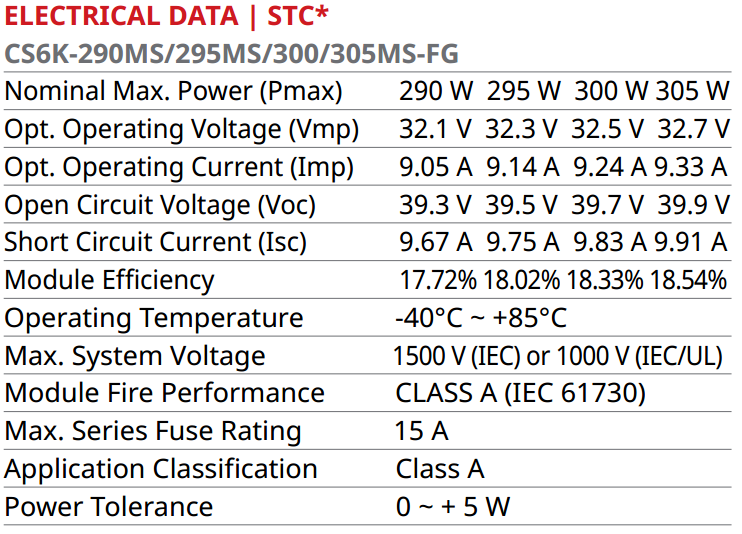
\includegraphics[width=0.55 \linewidth]{elet_canadian_300}
% 		\caption{Características elétricas em STC do painel modelo \cite{Canadian_Datasheet}}
% 		\label{fig:pv_elet}
% 	\end{center}
% \end{figure}

% Please add the following required packages to your document preamble:
% \usepackage{graphicx}
\begin{table}[H]
	\centering
	\resizebox{0.7 \textwidth}{!}{%
		\begin{tabular}{l|c|}
			\cline{2-2}
			\multicolumn{1}{c|}{}                                  & \textbf{CS6K 300}              \\ \hline
			\multicolumn{1}{|l|}{Potência máx. nominal (Pmax)}     & $300 W$                        \\ \hline
			\multicolumn{1}{|l|}{Tensão de operação ótima (Vmp)}   & $32,5V$                        \\ \hline
			\multicolumn{1}{|l|}{Corrente de operação ótima (Imp)} & $9,24 A$                       \\ \hline
			\multicolumn{1}{|l|}{Tensão de circuito aberto (Voc)}  & $39,7 V$                       \\ \hline
			\multicolumn{1}{|l|}{Corrente de curto circuito (Isc)} & $9,83 V$                       \\ \hline
			\multicolumn{1}{|l|}{Eficiência do módulo}             & $18,33\%$                      \\ \hline
			\multicolumn{1}{|l|}{Temperatura de operação}          & $-40^oC \sim +85^oC$          \\ \hline
			\multicolumn{1}{|l|}{Tensão máx. do sistema}           & 1500 (IEC) ou 1000 V (IEC/UL)  \\ \hline
			\multicolumn{1}{|l|}{Max. Series Fuse Rating 15 A}     & $15 A$                         \\ \hline
			\multicolumn{1}{|l|}{Classificação de operação}        & Classe A                       \\ \hline
			\multicolumn{1}{|l|}{Tolerância de potência}           & $0 \sim +5W$                \\ \hline
		\end{tabular}%
	}
	\caption{Características elétricas em STC\textsuperscript{\ref{foot_:STC}} do painel selecionado \cite{Canadian_Datasheet}}
	\label{tab:pv_elet}
\end{table}

% \begin{figure}[H]%
% 	\begin{center}%
% 		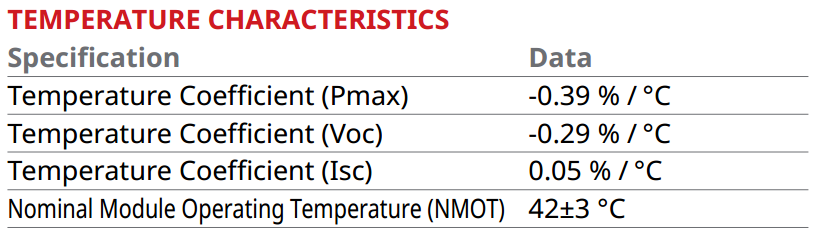
\includegraphics[width=0.55 \linewidth]{temp_canad_300}
% 		\caption{Características de temperatura do painel modelo \cite{Canadian_Datasheet}}
% 		\label{fig:pv_temp}
% 	\end{center}
% \end{figure}

% Please add the following required packages to your document preamble:
% \usepackage{graphicx}
\begin{table}[htb]
	\centering
	\resizebox{0.7 \textwidth}{!}{%
		\begin{tabular}{|l|c|}
			\hline
			Coeficiente de Temperatura (Pmax)                & $-0,39 ~\% / ^oC$ \\ \hline
			Coeficiente de Temperatura (Voc)                 & $-0,29~\% / ^oC$  \\ \hline
			Coeficiente de Temperatura (Isc)                 & $0,05~\% / ^oC$   \\ \hline
			Temperatura de Operação Nominal do Módulo (NMOT) & $42 \pm 3  ~^oC$  \\ \hline
		\end{tabular}%
	}
	\caption{Características de temperatura do painel selecionado \cite{Canadian_Datasheet}}
	\label{tab:pv_temp}
\end{table}

\begin{figure}[htb]%
	\begin{center}%
		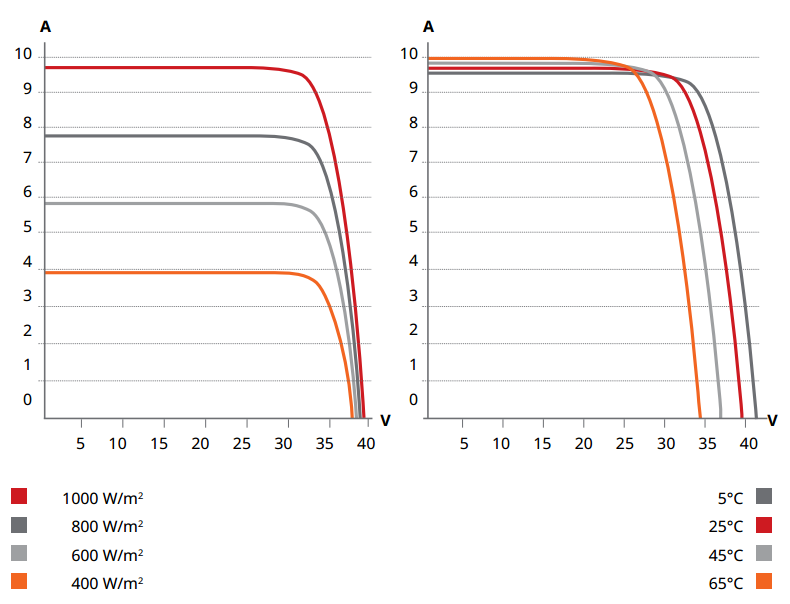
\includegraphics[width=0.7 \linewidth]{AV_canad_300}
		\caption{Curvas IxV do painel selecionado \cite{Canadian_Datasheet}}
		\label{fig:IV_pv_cs}
	\end{center}
\end{figure}

Para modelar o comportamento do painel no PSIM, foi seguido o procedimento indicado no tutorial \cite{PSIM_PV}. Utiliza-se, portanto, informações das presentes nas tabelas~\ref{tab:pv_elet} e \ref{tab:pv_temp}, já da figura~\ref{fig:IV_pv_cs} é extraída a inclinação $\frac{dV}{dI}$ na tensão de circuito aberto $V_{OC}$, que é de $-0,4 V/A$.

Nas figuras~\ref{fig:pv_psim_param} e \ref{fig:pv_psim_carac} são mostrados os parâmetros e as características, respectivamente, do módulo fotovoltaico utilizado no PSIM.

\begin{figure}[htb]%
	\begin{center}%
		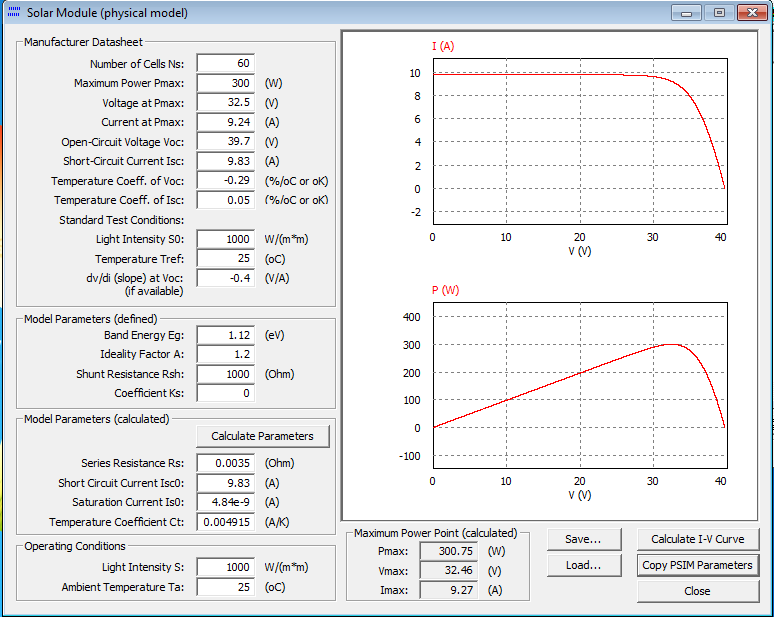
\includegraphics[width=0.7\linewidth]{PV_param}
		\caption{Parâmetros do módulo fotovoltaico no PSIM}
		\label{fig:pv_psim_param}
	\end{center}
\end{figure}

\begin{figure}[H]%
	\begin{center}%
		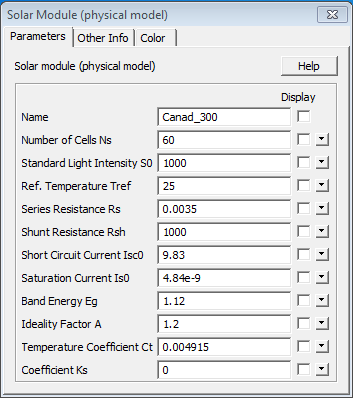
\includegraphics[width=0.55 \linewidth]{PV_carac}
		\caption{Características do módulo fotovoltaico no PSIM}
		\label{fig:pv_psim_carac}
	\end{center}
\end{figure}

O circuito que representa o painel fotovoltaico pode ser visto na figura~\ref{fig:pv_psim_circuit}, na qual \textit{Irrad} é a irradiância, \textit{Temp} a temperatura e $V_{out}$ a tensão de saída.

\begin{figure}[H]%
	\begin{center}%
		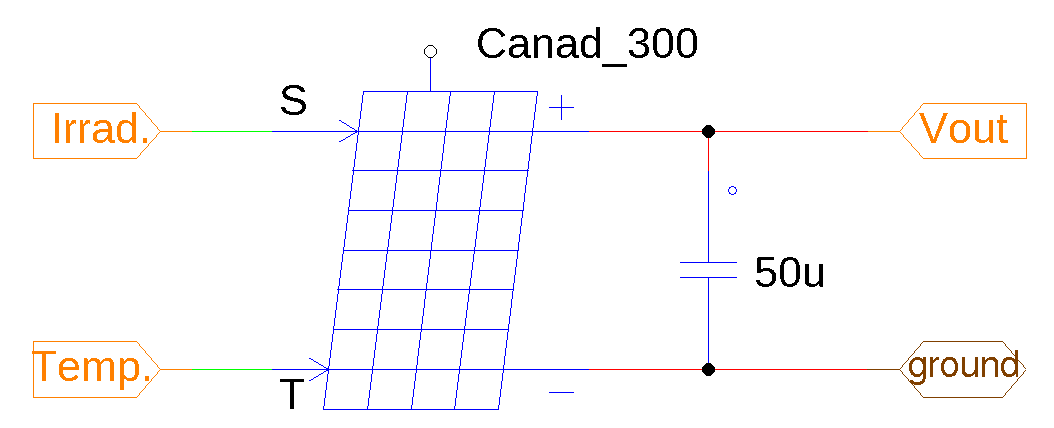
\includegraphics[width=0.65 \linewidth]{pv_psim_circuit}
		\caption{Circuito do módulo fotovoltaico no PSIM}
		\label{fig:pv_psim_circuit}
	\end{center}
\end{figure}


\section{Projeto dos Conversores CC/CC}

Apesar de mais complexos e caros que conversores CC/CC básicos, conversores cuk apresentam melhores características de corrente, tanto de entrada quanto de saída que estas topologias \cite{JOSEPH_2017_Intervealed_CUK} e, por isso foram escolhidos para como objeto de análise deste trabalho.

\subsection{Dimensionamento do Conversor Ćuk Convencional} \label{ssec:cuk_conv_met}

As seções~\ref{ssec:d_cuk_conv} a \ref{ssec:cap_cuk_conv} a seguir representam os passos no projeto de um conversor cuk convencional. Primeiramente é definido o comportamento desejado do circuito que, para este projeto é:

\begin{itemize}%
	\item Frequência de chaveamento de $15kHz$;
	\item Potência de $300W$;
	\item Tensão de entrada de $32,5V$, equivalente à tensão máxima do painel fotovoltaico;
	\item Tensão de saída de $180V$, equivalente à tensão de pico da rede elétrica monofásica;
	\item Tensão de ripple de saída de $0,5V$;
	\item Corrente de ripple de $0,1A$ no indutor $L2$;
	\item Tensão de ripple de $1V$ no capacitor de transferência $C1$;
	\item Corrente de ripple de $1A$ no indutor $L1$.
\end{itemize}

Além disso, dados a potência e tensão de saída pode-se encontrar a carga equivalente R:

\begin{equation}%
	R = \frac{P}{V^2} = 108 \Omega \label{eq:cuk_load}
\end{equation}

\subsubsection{Ciclo de Trabalho}\label{ssec:d_cuk_conv}

O ciclo de trabalho do conversor cuk é encontrado a partir de seus valores de tensão de entrada e saída desejados. Utilizando a função de transferência deste circuito, definida na equação~\ref{eq:trans_func_cuk_conv} e com as tensões de entrada e saída, encontra-se o \textit{duty cycle} encontrado na equação~\ref{eq:d_cuk_conv_}.

\begin{equation}%
	d = \frac{V_{o}}{V_{o}+V_{s}} = 0,847 \label{eq:d_cuk_conv_}
\end{equation}

\subsubsection{Indutores}

Para definir os indutores inicialmente é necessário encontrar o valor mínimo desses componentes para que o circuito opere em modo de condução contínua, através das equações~\ref{eq:cuk_conv_CCM_limits_l1} e \ref{eq:cuk_conv_CCM_limits_l2}. Sendo assim tem-se:

\begin{IEEEeqnarray}{c}
	L_{b1} = \frac{(1-d)R}{2 d f} = 648 \mu H \\
	L_{b2} = \frac{\left(1-d\right)R}{2 f}   = 549 \mu H 
\end{IEEEeqnarray}

Calcula-se, também, os valores necessários para obter o comportamento desejado do circuito e utiliza-se o menor valor que satisfaça as duas condições. Os cálculos para os parâmetros do circuito estão representados pelas equações~\ref{eq:cuk_conv_L1} e \ref{eq:cuk_conv_L2}.

\begin{IEEEeqnarray}{c}
	L1 = \frac{V_{s} \cdot d}{f \cdot 1,00A} = 1,99 mH \label{eq:cuk_conv_L1}\\
	L2 = \frac{V_{s} \cdot d}{f \cdot 0,10A} = 18,3 mH \label{eq:cuk_conv_L2}
\end{IEEEeqnarray}

\subsubsection{Capacitores}\label{ssec:cap_cuk_conv}

Os capacitores $C2$ e $C1$ são calculados a partir das equações~\ref{eq:rip_filt_conv_cuk} e \ref{eq:conv_cuk_rip_c1}, respectivamente. Substituindo os valores já encontrados nessas equações têm-se:

\begin{IEEEeqnarray}{c}
	C2 = \frac{0,153 \cdot 180V}{8 \cdot 0,5V \cdot 18,3mH  \cdot (15kHz)^2} = 1,67uF \\
	C1 = \frac{0,153 \cdot 180V}{108\Omega \cdot 15kHz \cdot 1V} = 94,3 uF \label{eq:cuk_conv_C1_final}
\end{IEEEeqnarray}

\subsubsection{Circuito resultante e resultados de simulação}

Com os valores de componentes calculados nas equações~\ref{eq:d_cuk_conv_} a \ref{eq:cuk_conv_C1_final}, ajustados para valores comerciais, foi montado o circuito de um conversor cuk convencional que pode ser visto na figura~\ref{fig:cuk_conv_psim_circ}.

\begin{figure}[htbp]%
	\captionsetup{justification=centering}
	\begin{center}%
		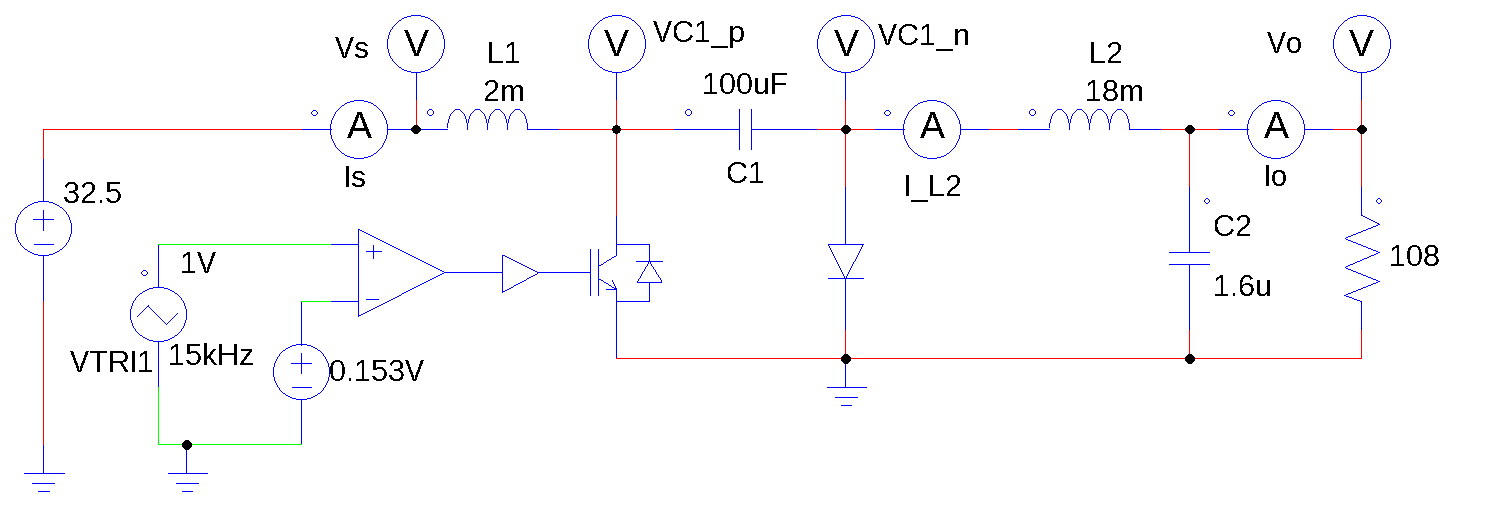
\includegraphics[width=0.95 \linewidth]{conv_cuk_psim_circ}
		\caption{Circuito do conversor cuk convencional com comando em malha aberta}
		\label{fig:cuk_conv_psim_circ}
	\end{center}
\end{figure}

A partir da simulação do circuito da figura~\ref{fig:cuk_conv_psim_circ} no PSIM, obteve-se os valores de média e ripple presentes na tabela~\ref{tab:conv_cuk_results}. Além disso, as formas de onda verificadas são apresentadas na figuras~\ref{fig:cuk_conv_ripp_I_L1} a \ref{fig:cuk_conv_power_sign}.

\begin{table}[htb]
	\centering
		\resizebox{0.5\linewidth}{!}{%
				\begin{tabular}{|
				>{\columncolor[HTML]{C0C0C0}}l |c|}
				\hline
				\textbf{Corrente média em $L1$}            			& 9,22A    \\ \hline
				\textbf{Corrente de ripple em $L1$}        			& 0,91A    \\ \hline
				\textbf{Corrente de ripple em $L2$}        			& 0,10A    \\ \hline
				\textbf{Tensão de ripple em $C1$}          			& 0,94V    \\ \hline
				\textbf{Tensão de saída média do conversor}     & -179,91V \\ \hline
				\textbf{Tensão de ripple de saída do conversor} & 0,53V    \\ \hline
				\textbf{Potência de saída média}                & 299,71W  \\ \hline
				\textbf{Oscilação da potência de saída}         & 1,77W    \\ \hline
				\end{tabular}%
		}
		\caption{Valores medidos para o conversor cuk convencional}
		\label{tab:conv_cuk_results}
	\end{table}

\begin{figure}[htb]%
	\centering
		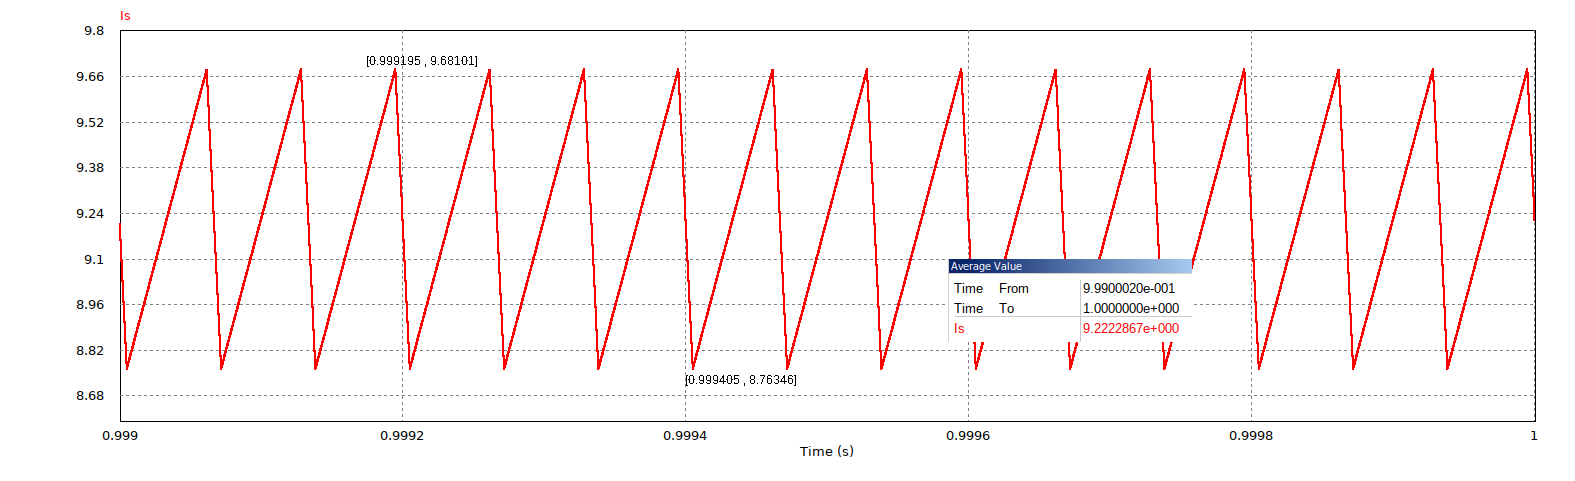
\includegraphics[width= \linewidth]{cuk_conv_ripp_I_L1}
		\caption{Corrente de ripple no indutor $L1$ do conversor cuk convencional}
		\label{fig:cuk_conv_ripp_I_L1}
\end{figure}

\begin{figure}[htb]%
	\centering
		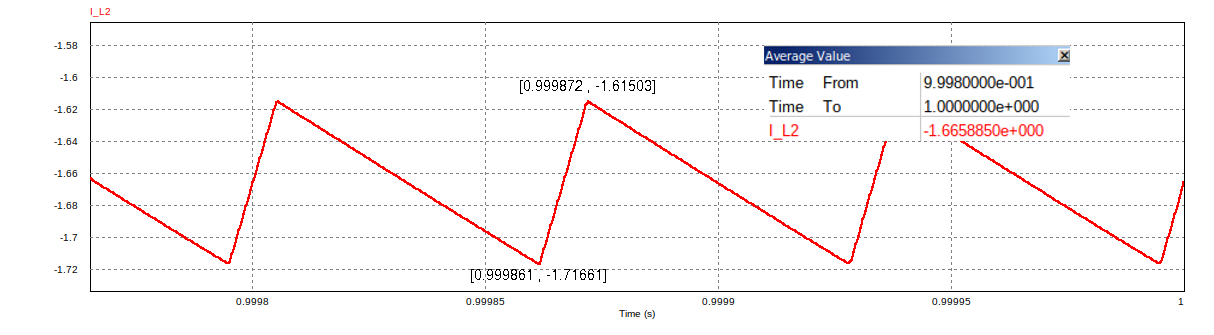
\includegraphics[width= \linewidth]{cuk_conv_ripp_I_L2}
		\caption{Corrente de ripple no indutor $L2$ do conversor cuk convencional}
		\label{fig:cuk_conv_ripp_I_L2}
\end{figure}

\begin{figure}[H]%
	\centering
		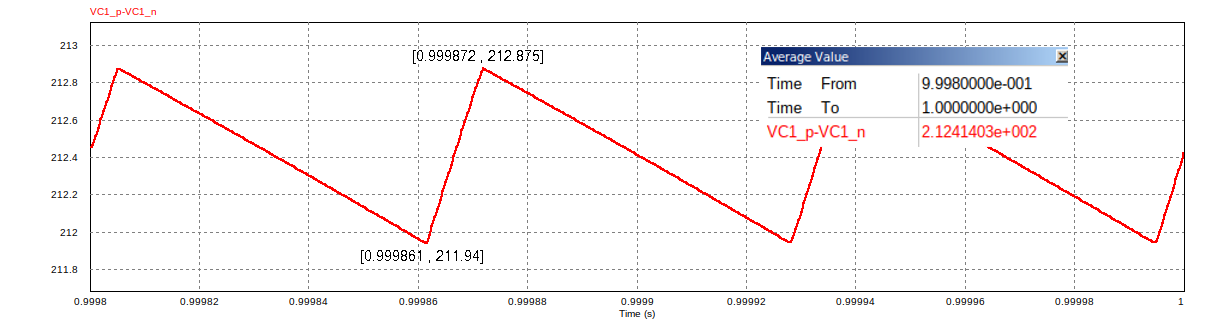
\includegraphics[width= \linewidth]{cuk_conv_ripp_V_C1}
		\caption{Tensão de ripple no capacitor $C1$ do conversor cuk convencional}
		\label{fig:cuk_conv_ripp_V_C1}
\end{figure}

% \begin{figure}[H]%
% 	\centering
% 		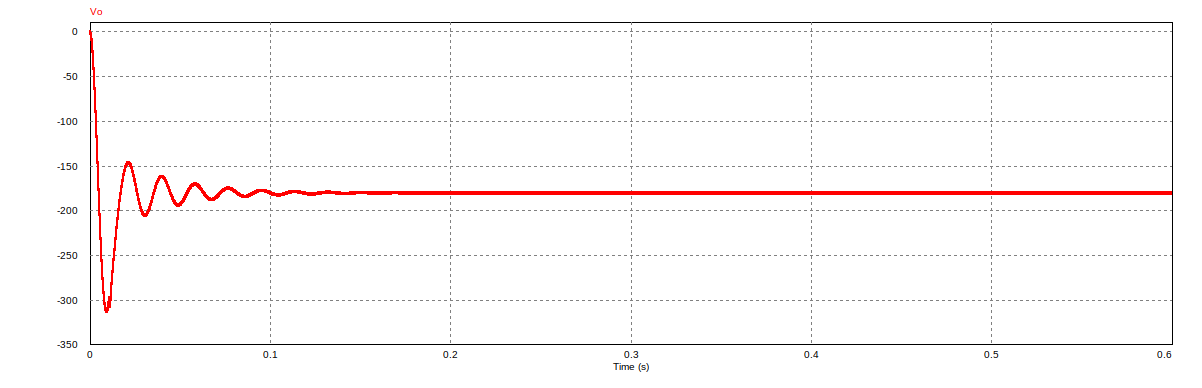
\includegraphics[width= \linewidth]{cuk_conv_V_out}
% 		\caption{Comportamento da tensão de saída do conversor cuk convencional}
% 		\label{fig:cuk_conv_V_out}
% \end{figure}

\begin{figure}[H]%
	\centering
		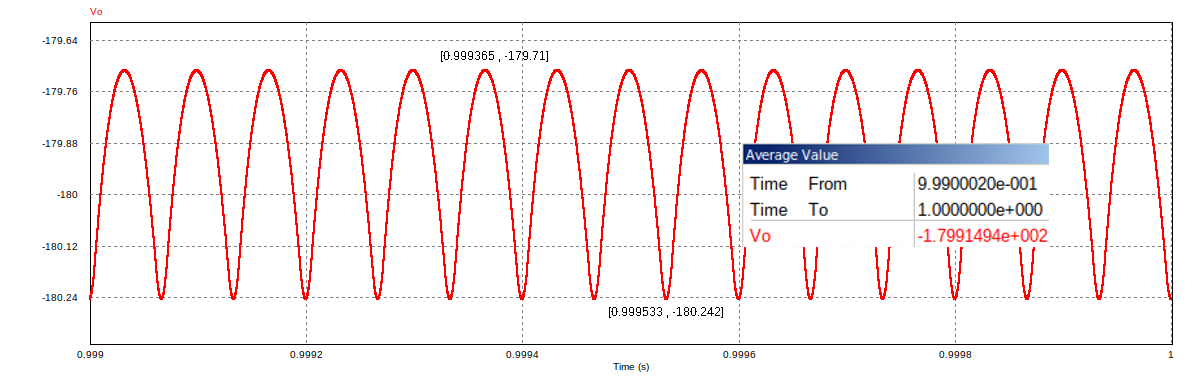
\includegraphics[width= \linewidth]{cuk_conv_ripp_V_out2}
		\caption{Tensão de saída do conversor cuk convencional}
		\label{fig:cuk_conv_ripp_V_out_}
\end{figure}

\begin{figure}[H]%
	\centering
		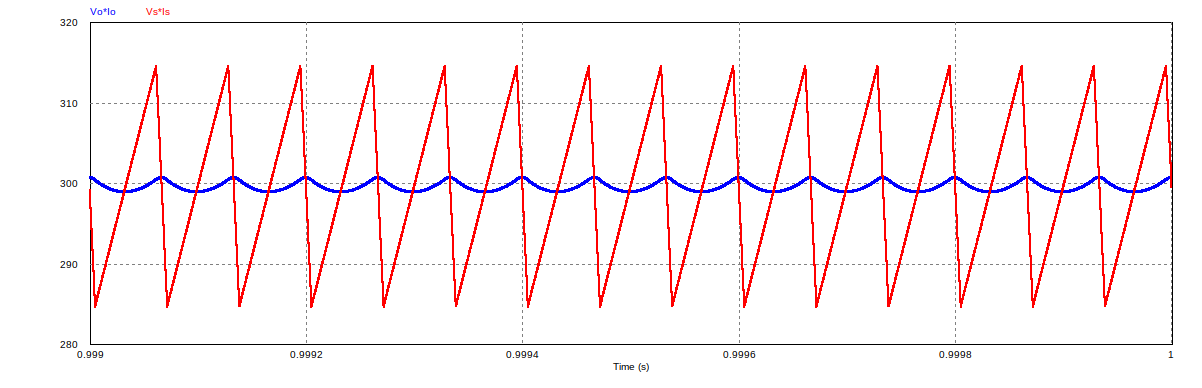
\includegraphics[width= \linewidth]{cuk_conv_power_sign}
		\caption{Potência na entrada e saída do conversor cuk convencional}
		\label{fig:cuk_conv_power_sign}
\end{figure}
% \vspace{-5pt}
% \begin{figure}[htb]%
% 	\centering
% 		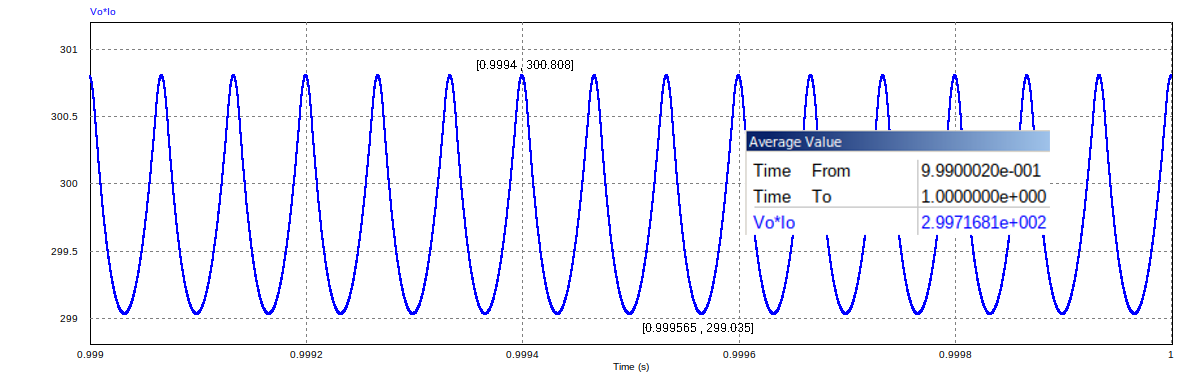
\includegraphics[width= \linewidth]{cuk_conv_power_sign_out}
% 		\caption{Oscilação da potência na saída do conversor cuk convencional}
% 		\label{fig:cuk_conv_power_sign_out}
% \end{figure}
% \vspace{-5pt}

Percebe-se, a partir dos dados expostos na tabela~\ref{tab:conv_cuk_results} que os ripples desejados foram atingidos. Além disso, o conversor projetado para 300W apresenta um ótimo rendimento, de 99,9\%, com uma oscilação de potência de apenas 0,6\%.


\subsection{Dimensionamento do Conversor Ćuk Entrelaçado}

O conversor cuk entrelaçado apresenta como principal vantagem ao conversor cuk convencional, menores ripples de corrente, já que a corrente de entrada é dividida entre as fases do mesmo \cite{JOSEPH_2015_Intervealed_CUK}\cite{JOSEPH_2017_Intervealed_CUK}. Essa característica também reduz o estresse de chaveamento dos transistores, implicando numa melhor qualidade da potência obtida e entregue pelo conversor \cite{JOSEPH_2017_Intervealed_CUK}.

Para a definição dos valores de componentes do conversor cuk entrelaçado serão utilizados os mesmos parâmetros de projeto do conversor cuk convencional. Além disso, os cálculos serão efetuados para uma das fases e os componentes encontrados serão replicados para todas as fases do circuito.

Dessa forma, a partir da equação~\ref{eq:cuk_load}, sabe-se que a carga equivalente vista pelo circuito $R$ é de $108\Omega$.

\subsubsection{Ciclo de Trabalho}

O ciclo de trabalho do conversor cuk entrelaçado é encontrado a partir da equação~\ref{eq:vo_interv} que equivale á equação ~\ref{eq:trans_func_cuk_conv}. Dessa forma, para os mesmos parâmetros de tensão de entrada e saída, o ciclo de trabalho deste conversor é igual ao do conversor cuk convencional, definido na equação~\ref{eq:d_cuk_conv_} como $0,847$.

\subsubsection{Indutores}

Como o ciclo de trabalho, a carga e a frequência de chaveamento do conversor cuk entrelaçado são iguais aos do conversor cuk convencional, os valores dos indutores a serem utilizados, por fase, serão iguais os encontrados para o conversor anterior. Dessa forma, teremos $L_{X1}$ e $L_{X2}$, onde $X$ indica a fase, definidos nas equações~\ref{eq:int_LX1} e \ref{eq:int_LX2}, respectivamente.
\begin{IEEEeqnarray}{c}%
	L_{X1} = 1,99mH \label{eq:int_LX1}\\
	L_{X2} = 18,3mH \label{eq:int_LX2}
\end{IEEEeqnarray}

\subsubsection{Capacitores}

Assim como no conversor cuk convencional, os capacitores são encontrados a partir das equações~\ref{eq:rip_filt_conv_cuk} e \ref{eq:conv_cuk_rip_c1}. Sendo assim, teremos os capacitores $C_{X1}$ e $C2$, onde $X$ representa a fase, com os valores presentes nas equações~\ref{eq:int_CX1} e \ref{eq:int_C2}, respectivamente.
\begin{IEEEeqnarray}{c}%
	C_{X1} = 1,67uF \label{eq:int_CX1}\\
	C2 = 94,3uF \label{eq:int_C2}
\end{IEEEeqnarray}

\subsubsection{Circuito resultante e resultados de simulação}

Assim como no conversor cuk convencional, os valores encontrados para cada componente foram aproximados a fim de se utilizar apenas valores comerciais. O circuito do conversor cuk entrelaçado de duas fases montado no PSIM pode ser visto na figura~\ref{fig:interv_cuk_conv_psim_circuit}.

Percebe-se que o pwm de cada braço, apesar de apresentar o mesmo ciclo de trabalho é defasado de $180^o$, que equivale ao atraso de $360^o/N$, onde N representa o número de fases~\cite{JOSEPH_2015_Intervealed_CUK}.

\begin{figure}[htbp]%
	\begin{center}%
		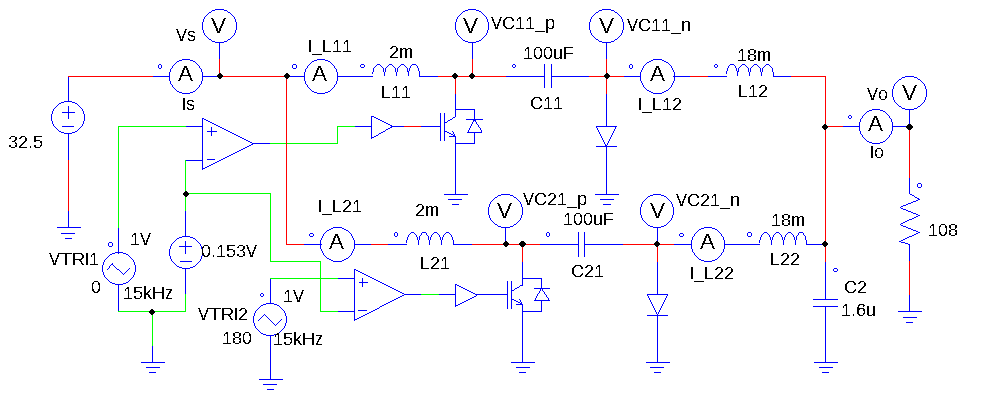
\includegraphics[width= \textwidth]{interv_cuk_psim_circ}
		\caption{Circuito do conversor cuk entrelaçado de duas fases}
		\label{fig:interv_cuk_conv_psim_circuit}
	\end{center}
\end{figure}

A partir da simulação do circuito da figura~\ref{fig:interv_cuk_conv_psim_circuit} no PSIM, obteve-se os valores de média e ripple presentes na tabela~\ref{tab:inter_cuk_results}. Além disso, as formas de onda verificadas são apresentadas na figuras~\ref{fig:cuk_inter_ripp_I_L1} a \ref{fig:cuk_inter_power_sign_out}.\

\begin{table}[htbp]
	\centering
		\resizebox{0.6\linewidth}{!}{%
		\begin{tabular}{l|c|c|c|}
				\cline{2-4}
																																																			& Fase 1 & Fase 2 & -					\\ \hline
				\multicolumn{1}{|l|}{\cellcolor[HTML]{C0C0C0}\textbf{Corrente média em $L_{X1}$}}             & 4,62A  & 4,60A  & -					\\ \hline
				\multicolumn{1}{|l|}{\cellcolor[HTML]{C0C0C0}\textbf{Corrente de ripple em $L_{X1}$}}         & 0,91A  & 0,90A  & -					\\ \hline
				\multicolumn{1}{|l|}{\cellcolor[HTML]{C0C0C0}\textbf{Corrente de ripple em $L_{X2}$}}         & 0,10A  & 0,10A  & -					\\ \hline
				\multicolumn{1}{|l|}{\cellcolor[HTML]{C0C0C0}\textbf{Tensão de ripple em $C_{X1}$}}           & 0,83V  & 0,83A  & -					\\ \hline
				\multicolumn{1}{|l|}{\cellcolor[HTML]{C0C0C0}\textbf{Corrente média na entrada}}              & -      & -      & 9,22A			\\ \hline
				\multicolumn{1}{|l|}{\cellcolor[HTML]{C0C0C0}\textbf{Corrente de ripple na entrada}}          & -      & -      & 0,74A   	\\ \hline
				\multicolumn{1}{|l|}{\cellcolor[HTML]{C0C0C0}\textbf{Tensão média de saída do conversor}}     & -      & -      & -179,91V	\\ \hline
				\multicolumn{1}{|l|}{\cellcolor[HTML]{C0C0C0}\textbf{Tensão de ripple de saída do conversor}} & -      & -      & 0,22V   	\\ \hline
				\multicolumn{1}{|l|}{\cellcolor[HTML]{C0C0C0}\textbf{Potência de saída média}}                & -      & -      & 299,71W 	\\ \hline
				\multicolumn{1}{|l|}{\cellcolor[HTML]{C0C0C0}\textbf{Oscilação da potência de saída}}         & -      & -      & 0,72W   	\\ \hline
			\end{tabular}%
		}
		\caption{Valores medidos para o conversor cuk entrelaçado de duas fases}
		\label{tab:inter_cuk_results}
	\end{table}

\begin{figure}[htb]%
	\captionsetup{justification=centering}
	\centering
		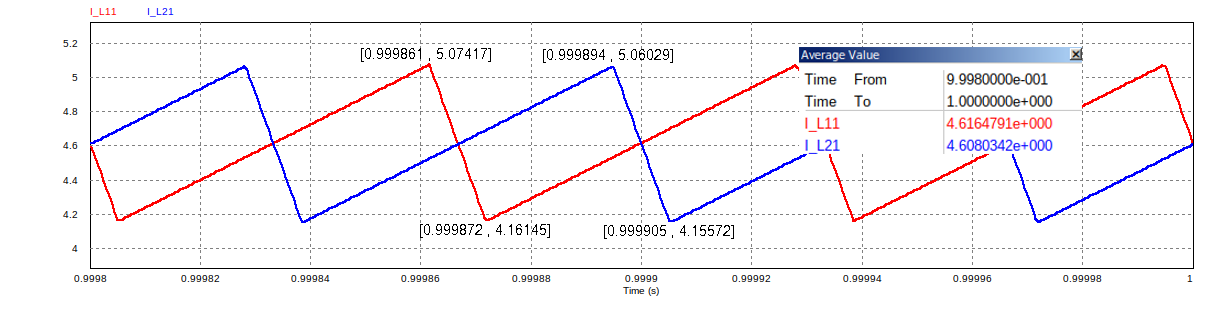
\includegraphics[width= \linewidth]{cuk_inter_ripp_I_LX1}
		\caption{Corrente de ripple no indutores $L_{11}$ e $L_{21}$ do conversor cuk entrelaçado de duas fases}
		\label{fig:cuk_inter_ripp_I_L1}
\end{figure}

\begin{figure}[htb]%
	\captionsetup{justification=centering}
	\centering
		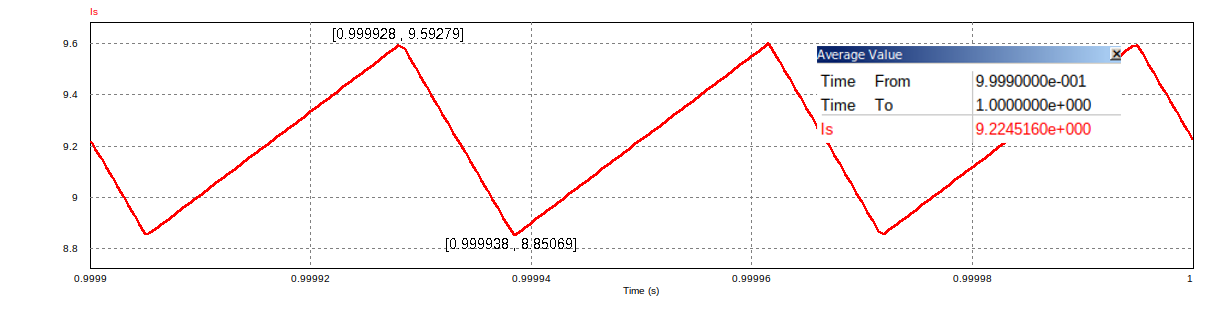
\includegraphics[width= \linewidth]{cuk_inter_ripp_I_S}
		\caption{Corrente de ripple na entrada do conversor cuk entrelaçado de duas fases}
		\label{fig:cuk_inter_ripp_I_S}
\end{figure}

\begin{figure}[htb]%
	\captionsetup{justification=centering}
	\centering
		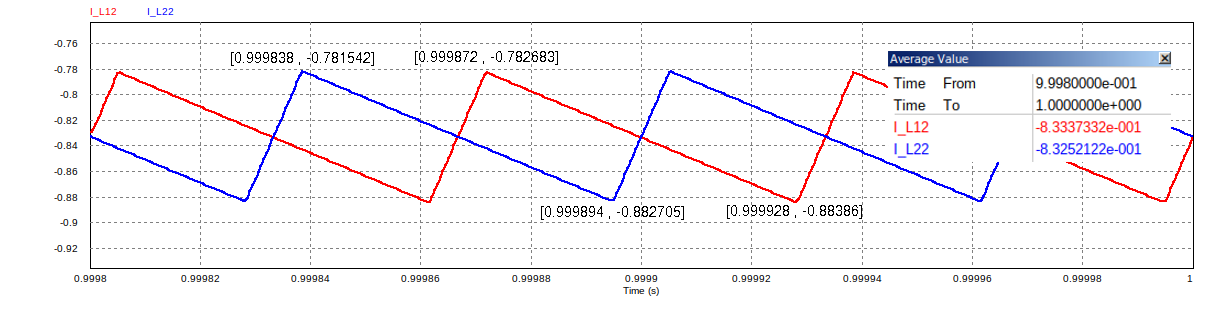
\includegraphics[width= \linewidth]{cuk_inter_ripp_I_LX2}
		\caption{Corrente de ripple nos indutores $L_{12}$ e $L_{22}$ do conversor cuk entrelaçado de duas fases}
		\label{fig:cuk_inter_ripp_I_L2}
\end{figure}

\begin{figure}[H]%
	\captionsetup{justification=centering}
	\centering
		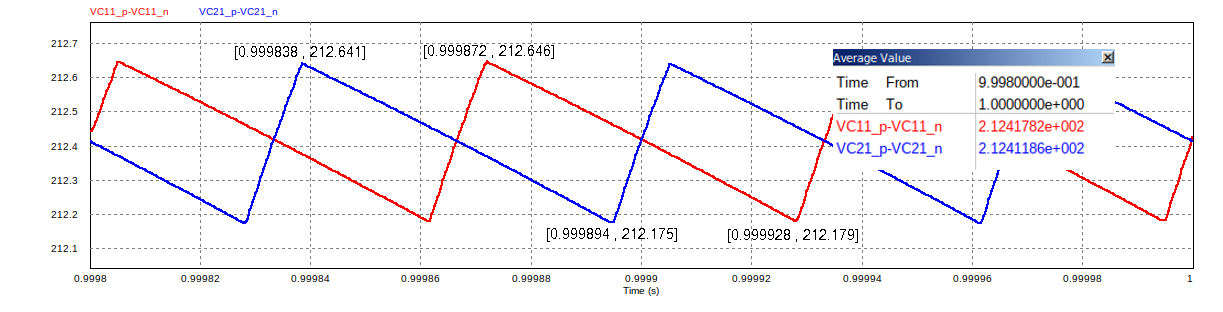
\includegraphics[width= \linewidth]{cuk_inter_ripp_V_CX1}
		\caption{Tensão de ripple nos capacitores $C_{11}$ e $C_{21}$ do conversor cuk entrelaçado de duas fases}
		\label{fig:cuk_inter_ripp_V_C1}
\end{figure}

% \begin{figure}[H]%
% 	\captionsetup{justification=centering}
% 	\centering
% 		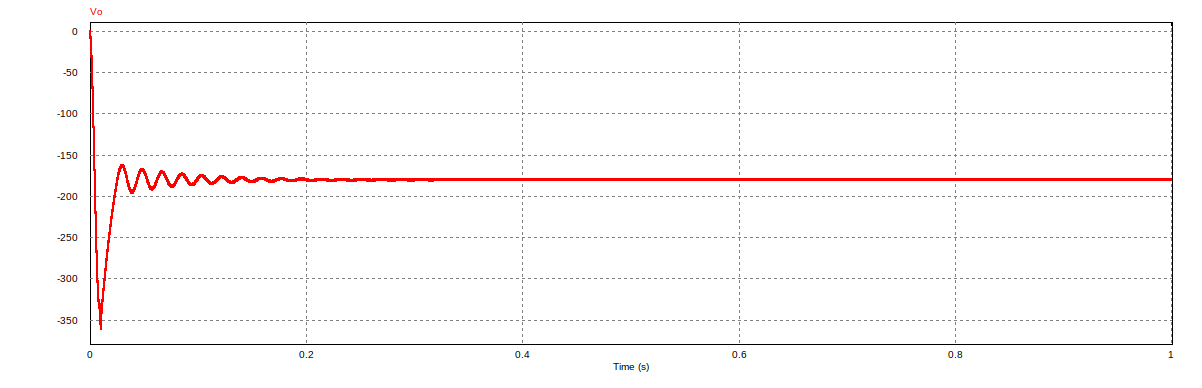
\includegraphics[width= \linewidth]{cuk_inter_V_out}
% 		\caption{Comportamento da tensão de saída do conversor cuk entrelaçado de duas fases}
% 		\label{fig:cuk_inter_V_out}
% \end{figure}

\begin{figure}[H]%
	\captionsetup{justification=centering}
	\centering
		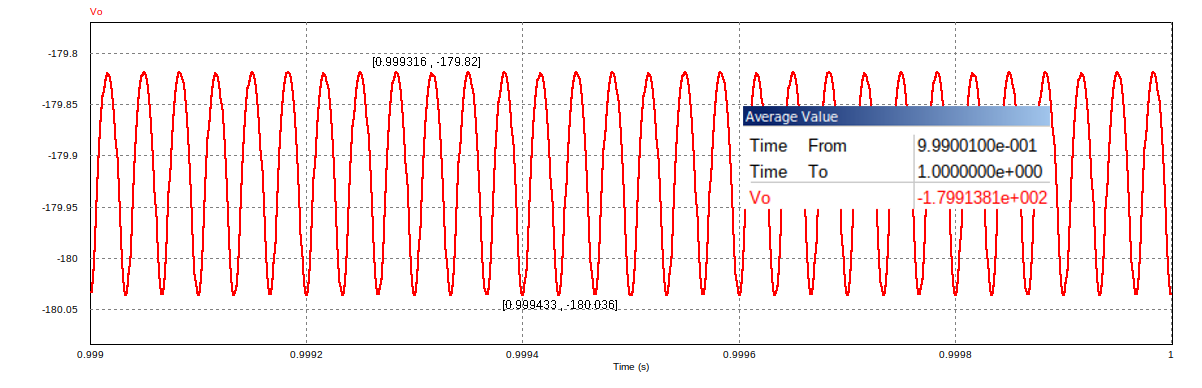
\includegraphics[width= \linewidth]{cuk_inter_ripp_V_out}
		\caption{Tensão de ripple de saída do conversor cuk entrelaçado de duas fases}
		\label{fig:cuk_inter_ripp_V_out}
\end{figure}

\begin{figure}[H]%
	\captionsetup{justification=centering}
	\centering
		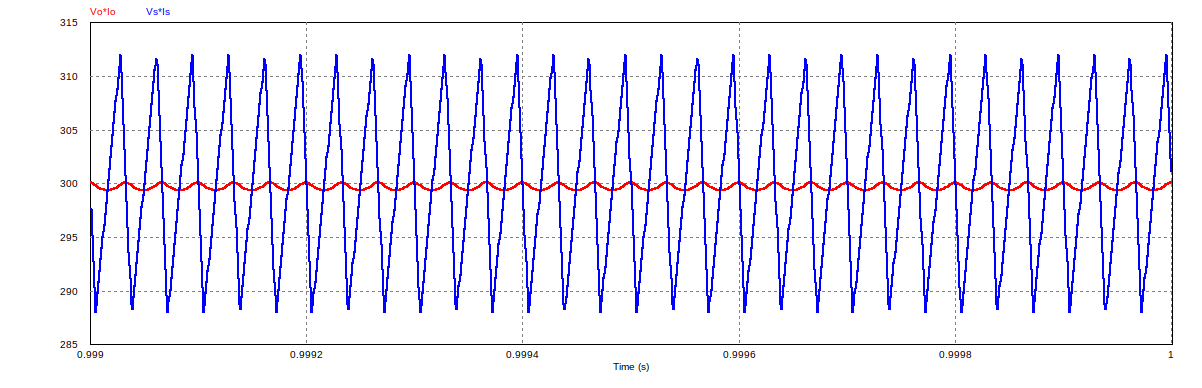
\includegraphics[width= \linewidth]{cuk_inter_power_sign}
		\caption{Potência na entrada e saída do conversor cuk entrelaçado de duas fases}
		\label{fig:cuk_inter_power_sign}
\end{figure}

\begin{figure}[H]%
	\captionsetup{justification=centering}
	\centering
		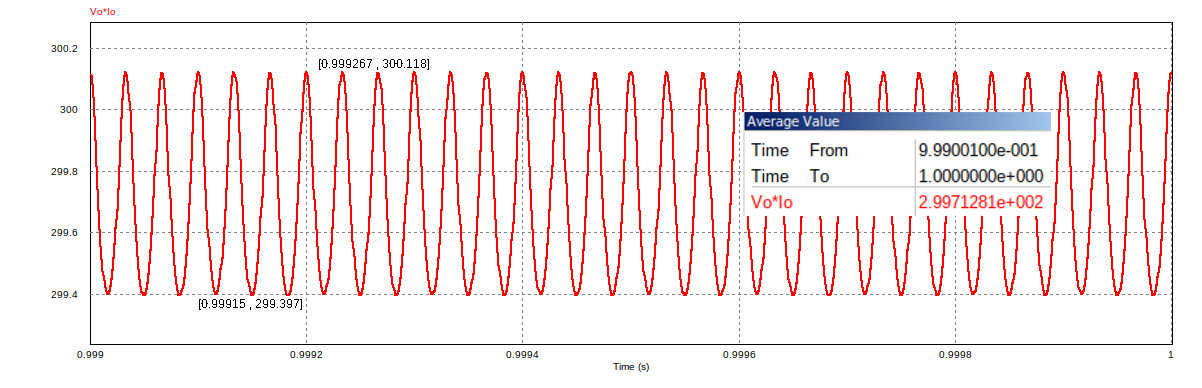
\includegraphics[width= \linewidth]{cuk_inter_pow_out}
		\caption{Oscilação da potência saída do conversor cuk entrelaçado de duas fases}
		\label{fig:cuk_inter_power_sign_out}
\end{figure}

De acordo com os resultados presentes na tabela~\ref{tab:inter_cuk_results}, foram obtidos os valores desejados cada uma das fases do conversor. Se comparados aos valores referentes aos resultados do conversor cuk convencional, tabela~\ref{tab:conv_cuk_results}, é possível perceber que, enquanto cada uma das fases do conversor cuk entrelaçado apresenta ripple de corrente igual ao encontrado na entrada do conversor cuk convencional, a variação da corrente na entrada do conversor cuk entrelaçado é equivalente a 78\% da encontrada na outra implementação.

Além da melhoria de qualidade da corrente de entrada no circuito, o conversor cuk entrelaçado também apresentou tensão de ripple equivalente a 58\% menor e oscilação de potência equivalente a 41\% dos valores apresentados pela implementação convencional, apesar de apresentar mesmo rendimento que este, considerando-se valores médios de potência.

\section{Projeto dos Conversores CC/CA} \label{sec:met_conv_cc_ca}

\subsection{Inversor tipo fonte de tensão (\textit{VSI}) Bipolar}

A figura~\ref{fig:VSI_bip_circ} apresenta o circuito montado no PSIM para simular um inversor VSI com PWM bipolar. Foi utilizada uma fonte de tensão de $180V$ para emular a alimentação do circuito.

Para o sinal de portadora foi utilizada uma fonte de sinal triangular de 1kHz e $3V$ de amplitude pico a pico. Já como modulante, uma fonte de sinal senoidal de $1V$ e 60Hz, uma vez que a modulante deve corresponder à forma de onda e frequência da saída desejada.

\begin{figure}[htpb]%
	\centering%
		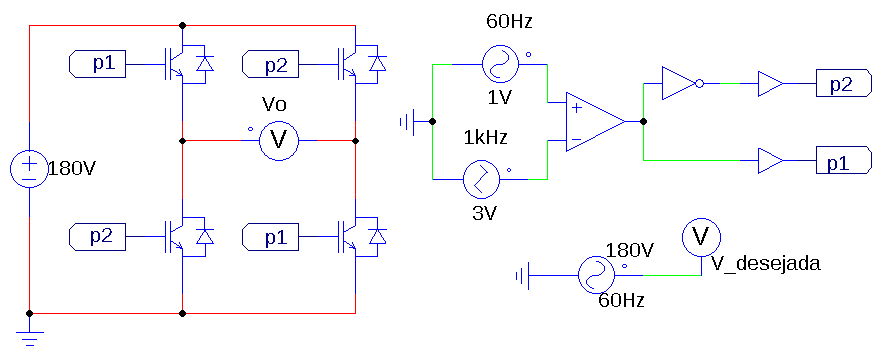
\includegraphics[width=0.8 \linewidth]{vsi_bipolar_psim_circ}
		\caption{Inversor VSI Bipolar em malha aberta}
		\label{fig:VSI_bip_circ}
\end{figure}

Para analisar as características deste inversor foi simulado o circuito da figura~\ref{fig:VSI_bip_circ}, do qual obteve-se o sinal de saída que pode ser visto na figura~\ref{fig:response_vsi_bip}, juntamente com o sinal senoidal desejado, para facilitar a comparação. Ainda na figura~\ref{fig:response_vsi_bip} é possível verificar que este circuito apresenta distorção harmônica total, \emph{THD}, do inglês \textit{Total Harmonic Distortion} de $1,84\%$.

\begin{figure}[htbp]%
	\centering
		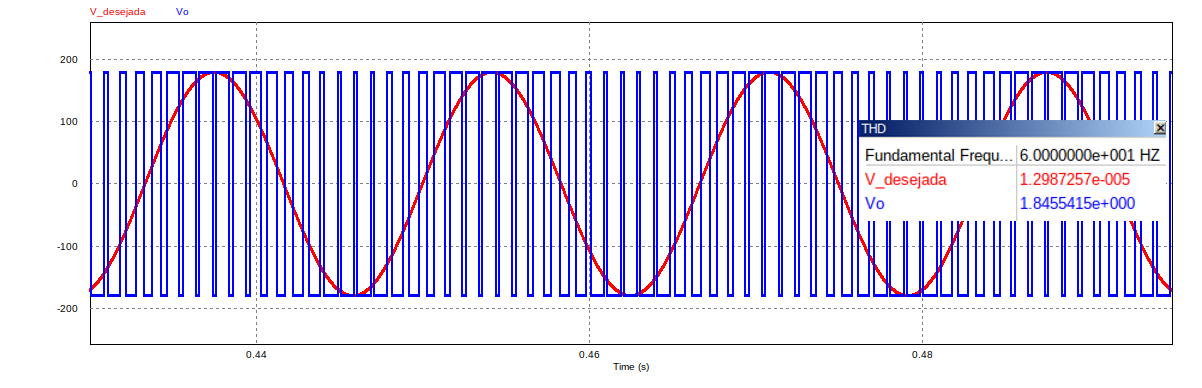
\includegraphics[width= \linewidth]{vsi_bip_out}
		\caption{Sinal de saída do inversor VSI bipolar}
		\label{fig:response_vsi_bip}
\end{figure}

\subsection{Inversor tipo fonte de tensão (\textit{VSI}) Unipolar}

A figura~\ref{fig:VSI_uni_circ} apresenta o circuito montado no PSIM para simular um inversor VSI com PWM unipolar. Assim como no inversor bipolar, utilizou-se uma fonte de tensão contínua de $180V$ para emular a alimentação do circuito.

Para o sinal de portadora foi utilizada uma fonte de sinal triangular de 1kHz e $3V$ de amplitude pico a pico. Já para as modulantes, foram utilizadas duas fontes senoidais de 60Hz e $1V$ de amplitude, defasadas entre si de $180^o$.

\begin{figure}[H]%
	\centering%
		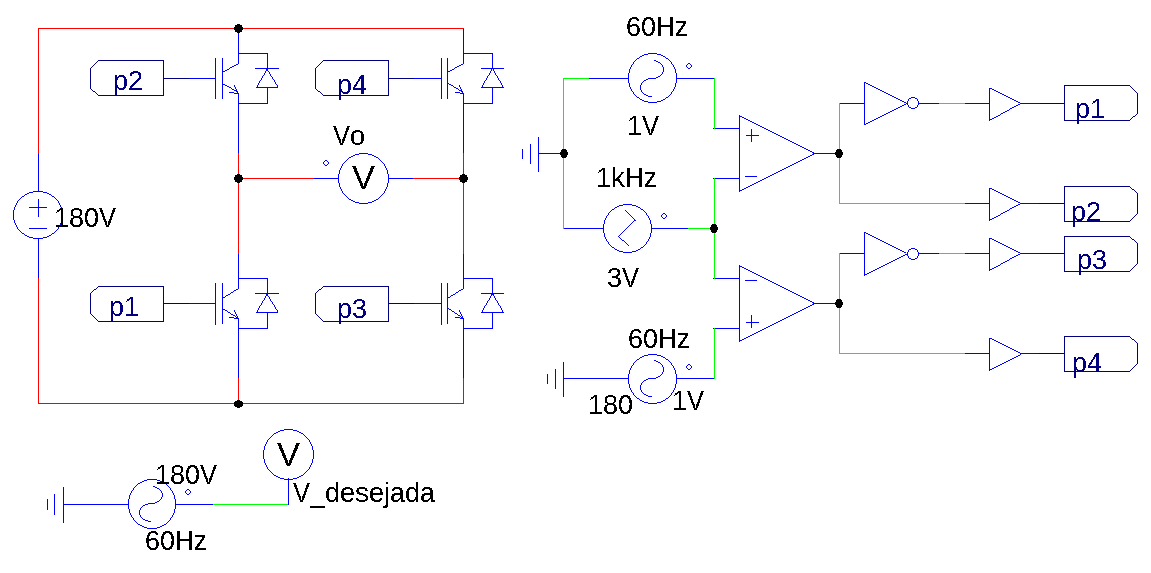
\includegraphics[width=0.85 \linewidth]{vsi_unipolar_psim_circ}
		\caption{Inversor VSI Unipolar}
		\label{fig:VSI_uni_circ}
\end{figure}

Para analisar as características deste inversor foi simulado o circuito da figura~\ref{fig:VSI_uni_circ}, do qual assim como para o inversor bipolar, obteve-se o sinal de saída, presente na figura~\ref{fig:response_vsi_uni}. Ainda a partir desta figura verifica-se que este circuito apresenta distorção harmônica total consideravelmente inferior ao inversor bipolar, de $0,96\%$.

\begin{figure}[H]%
	\centering
		\includegraphics[width= \linewidth]{vsi_uni_out}
		\caption{Sinal de saída do inversor VSI unipolar}
		\label{fig:response_vsi_uni}
\end{figure}

% \section{Inversor Integrado (CC/CA)}\label{sec:met_conv_integ}
\subsection{Inversor Ćuk Integrado}

O inversor cuk integrado é uma versão simplificada do conversor convencional, descrito na seção~\ref{ssec:cuk_conv_met}. Nesta implementação, os componentes responsáveis pela filtragem do sinal de saída ($L2$ e $C2$) e é incorporado ao capacitor $C1$ um inversor. Os diodos paralelos aos transistores do inversor executam a função do diodo.

Dessa forma, tanto o ciclo de trabalho quanto os valores dos componentes restantes, $L1$ e $C1$ podem ser encontrados através das equações do conversor cuk convencional, sendo estas as equações~\ref{eq:d_cuk_conv_}, \ref{eq:cuk_conv_L1} e \ref{eq:cuk_conv_C1_final}, respectivamente.

\subsubsection{Circuito Resultante e resultados de simulação}

Sendo assim está presente na figura~\ref{fig:integ_cuk_met} o circuito utilizado na simulação do inversor cuk integrado.
% As figuras~\ref{fig:cuk_integ_I_L1} a \ref{fig:cuk_integ_ripp_V_C1} representam os sinais de entrada e saída do inversor cuk integrado.

\begin{figure}[htbp]%
	\begin{center}%
		\includegraphics[width= \linewidth]{integ_cuk_circ_psim}
		\caption{Circuito do inversor cuk integrado}
		\label{fig:integ_cuk_met}
	\end{center}
\end{figure}

\begin{figure}[htb]%
	\centering
		\includegraphics[width= \linewidth]{cuk_integ_Vout}
		\caption{Sinal de saída do inversor cuk integrado}
		\label{fig:cuk_integ_ripp_V_out}
\end{figure}

\begin{figure}[htb]%
	\centering
		\includegraphics[width= \linewidth]{cuk_integ_IL1}
		\caption{Corrente no indutor $L1$ do inversor cuk integrado}
		\label{fig:cuk_integ_I_L1}
\end{figure}

\begin{figure}[htb]%
	\centering
		\includegraphics[width= \linewidth]{cuk_integ_ripp_IL1}
		\caption{Detalhe da oscilação na corrente no indutor $L1$ do inversor cuk integrado}
		\label{fig:cuk_integ_ripp_I_L1}
\end{figure}

\begin{figure}[H]%
	\centering
		\includegraphics[width= \linewidth]{cuk_integ_VC1}
		\caption{Tensão no capacitor $C1$ do inversor cuk integrado}
		\label{fig:cuk_integ_V_C1}
\end{figure}

\begin{figure}[H]%
	\centering
		\includegraphics[width= \linewidth]{cuk_integ_ripp_VC1}
		\caption{Detalhe da oscilação na tensão no capacitor $C1$ do inversor cuk integrado}
		\label{fig:cuk_integ_ripp_V_C1}
\end{figure}

Nas figuras~\ref{fig:cuk_integ_I_L1} a \ref{fig:cuk_integ_ripp_V_C1} é possível perceber a influência do chaveamento dos transistores do inversor utilizado nos sinais da corrente de entrada e da tensão no capacitor $C1$, que apresentam um ruído triangular de alta frequência de aproximadamente 0,91A e 0,57V, respectivamente além de características senoidais.


\section{Rastreador de ponto de máxima potência (\textit{MPPT})}\label{sec:met_mppt}

O algoritmo de rastreamento de ponto de máxima potência do painel fotovoltaico escolhido foi o \textit{P\&O}. Foi desenvolvida uma rotina em C, que segue o fluxograma da figura~\ref{fig:PeO_Flux} utilizando o \textbf{C Block}, um segurador de ordem zero com frequência de amostragem de $500Hz$ e um comparador de tensão ao qual é conectado uma fonte de sinal triangular de $15kHz$ e $1V$ de amplitude, a portadora.

O segurador se faz necessário para determinar a frequência da execução da rotina, uma vez que o \textbf{C Block} executa o código a cada passo da simulação.

Para facilitar a inserção da MPPT nos circuitos, foi montado um sub-circuito, que compreende os dois blocos e o comparador da implementação(\ref{fig:mppt_subcircuit}). O código implementado pode ser visto no anexo~\ref{anex:mppt_code}.

\begin{figure}[htb]%
	\begin{center}%
		\includegraphics[width=0.85 \linewidth]{mppt_psim_circ}
		\caption{Circuito de MPPT implementado}
		\label{fig:mppt_subcircuit}
	\end{center}
\end{figure}

Nas figuras~\ref{fig:mppt_conv_data} e \ref{fig:mppt_interv_data} são expostos os comportamentos dos conversores cuk convencional e entrelaçado de duas fases quando alimentados pelo painel fotovoltaico juntamento com o MPPT implementado. Os circuitos utilizados podem ser vistos nas figuras~\ref{fig:mppt_conv_circ} e \ref{fig:mppt_interv_circ}.

\begin{figure}[htb]%
	\captionsetup{justification=centering}%
	\begin{center}%
		\includegraphics[width= \linewidth]{mppt_conv_circ}
		\caption{Circuito do conversor cuk convencional alimentado pelo painel fotovoltaico com MPPT}
		\label{fig:mppt_conv_circ}
	\end{center}
\end{figure}

\begin{figure}[htb]%
	\captionsetup{justification=centering}%
	\begin{center}%
		\includegraphics[width= \textwidth]{mppt_conv_data}
		\caption{Comportamento do ciclo de trabalho e da potência de saída para alterações de irradiância para o conversor cuk convencional}
		\label{fig:mppt_conv_data}
	\end{center}
\end{figure}

\begin{figure}[htb]%
	\captionsetup{justification=centering}%
	\begin{center}%
		\includegraphics[width= \linewidth]{mppt_interv_circ}
		\caption{Circuito do conversor cuk entrelaçado alimentado pelo painel fotovoltaico com MPPT}
		\label{fig:mppt_interv_circ}
	\end{center}
\end{figure}

\begin{figure}[H]%
	\captionsetup{justification=centering}%
	\begin{center}%
		\includegraphics[width= \textwidth]{mppt_interv_data}
		\caption{Comportamento do ciclo de trabalho e da potência de saída para alterações de irradiância para o conversor cuk entrelaçado}
		\label{fig:mppt_interv_data}
	\end{center}
\end{figure}

\section{Filtro}\label{sec:met_filt}

Os componentes do filtro são encontrados a partir das equações~\ref{eq:lcl_zb} a \ref{eq:lcl_rf}.

O filtro é projetado para um inversor de $300W$, conectado a rede monofásica, com tensão de barramento CC de $210V$ e frequência de chaveamento de $15kHz$. Utilizando esses parâmetros, são encontrados os componentes representados pelas equações~\ref{eq:lcl_l1_met} a \ref{eq:lcl_c_met}.
\begin{IEEEeqnarray}{c}%
	L_1 = 9,88mH \label{eq:lcl_l1_met}\\
	L_2 = 68,4 \mu H \label{eq:lcl_l2_met}\\
	C = 9,87uF \label{eq:lcl_c_met}
\end{IEEEeqnarray}

Verifica-se, a partir da equação~\ref{eq:lcl_fres} e dos componentes encontrados que a frequência de ressonância do circuito é de $6144Hz$. Como a frequência de ressonância é superior a $600Hz$ e inferior a $7500Hz$ a equação~\ref{eq:lcl_fres_law} é satisfeita e pode-se calcular o resistor de ressonância, a partir da equação~\ref{eq:lcl_rf}. O valor encontrado para o resistor está presente na equação~\ref{eq:lcl_rf_met}.
\begin{equation}%
	R_f = 0,87 \Omega \label{eq:lcl_rf_met}
\end{equation}

O filtro resultante pode ser visto na figura~\ref{fig:lcl_filter_impl}, com o capacitor $C$ aproximado para o valor comercial mais próximo, de $10 \mu F$.

\begin{figure}[H]%
	\begin{center}%
		\includegraphics[width=0.65 \linewidth]{lcl_filter_psim}
		\caption{Filtro LCL implementado}
		\label{fig:lcl_filter_impl}
	\end{center}
\end{figure}

\chapter{Implementação dos conversores finais}

Neste capítulo são apresentados os conversores formados a partir da conexão dos circuitos dimensionados no capítulo~\ref{cap:project} e os resultados das simulações executadas com os mesmos.

São, ao todo, seis conjuntos distintos uma vez que cada implementação proposta é conectada a um inversor bipolar e a um inversor unipolar, a fim de avaliar a influência desse estágio. Todos as combinações apresentam, entretanto, o painel fotovoltaico, o rastreador de ponto máximo de potência e o filtro LCL em comum.

Todas as figuras de circuitos desse capítulo são apresentadas também no anexo~\ref{anex:circ_images} em modo paisagem e, portanto, com maior qualidade.

\subsection{Conjuntos baseados no conversor cuk convencional}
% \subsubsection{Conversor Ćuk Convencional com Inversor VSI Bipolar}
\subsubsection{Inversor cuk convencional bipolar}

O circuito implementado no PSIM para o conjunto que utiliza o conversor cuk convencional conectado ao inversor bipolar, com rastreamento de ponto máximo de potência é apresentado na figura~\ref{fig:comp_conv_circ_clean}. Além disso, a tabela~\ref{tab:conv_bip_res} apresenta os principais resultados encontrados através da simulação deste circuito.

Na figura~\ref{fig:out_conv_bip} são apresentados tensão e corrente de saída, ampliada em dez vezes. O espectro de frequências da tensão de saída obtida pode ser analisada na figura~\ref{fig:fft_conv_bip},  com informação da distorção harmônica total da tensão, considerando frequência base de 60Hz.

Já a figura~\ref{fig:comp_conv_var_s_bip} mostra os sinais de entrada e saída do conjunto para alterações na irradiância que alimenta o painel fotovoltaico.

\begin{figure}[H]%
	\captionsetup{justification=centering}
	\centering
		\includegraphics[width= \linewidth]{comp_conv_circ_clean}
		\caption{Circuito implementado para o inversor cuk convencional bipolar}
		\label{fig:comp_conv_circ_clean}
\end{figure}

\begin{table}[H]
	\captionsetup{justification=centering}
	\centering
	\resizebox{\textwidth}{!}{%
		\begin{tabular}{|l|l|l|l|l|l|l|}
		\hline
		\rowcolor[HTML]{C0C0C0} 
		\textbf{Corrente de saída eficaz} & \textbf{Corrente de ripple}   & \textbf{Tensão de saída eficaz} & \textbf{Tensão de Ripple}   & \textbf{Potência de saída}    & \textbf{Rendimento}   & \textbf{THD}                \\ \hline
		\multicolumn{1}{|c|}{$2,26 A$}      & \multicolumn{1}{c|}{$20,21 mA$} & \multicolumn{1}{c|}{$126,55 V$}   & \multicolumn{1}{c|}{$1,13 V$} & \multicolumn{1}{c|}{$286,00 W$} & \multicolumn{1}{c|}{$95,33\%$} & \multicolumn{1}{c|}{$1,20\%$} \\ \hline
		\end{tabular}%
	}
	\caption{Valores obtidos para o inversor cuk convencional bipolar}
	\label{tab:conv_bip_res}
\end{table}

\begin{figure}[H]%
	\captionsetup{justification=centering}
	\centering
		\includegraphics[width= \linewidth]{conv_Vo_10Io_comp}
		\caption{Sinais de saída obtidos para o inversor cuk convencional bipolar}
		\label{fig:out_conv_bip}
\end{figure}

\begin{figure}[H]%
	\captionsetup{justification=centering}
	\centering
		\includegraphics[width= \linewidth]{fft_conv_bip_2}
		\caption{Espectro de frequências da tensão de saída do inversor cuk convencional bipolar}
		\label{fig:fft_conv_bip}
\end{figure}

\begin{figure}[H]%
	\captionsetup{justification=centering}
	\centering
		\includegraphics[width= \linewidth]{comp_conv_var_s}
		\caption{Sinais de entrada e saída para o inversor cuk convencional bipolar com variação de irradiância}
		\label{fig:comp_conv_var_s_bip}
\end{figure}

\subsubsection{Inversor cuk convencional unipolar}

O circuito implementado no PSIM para o conjunto que utiliza o conversor cuk convencional conectado ao inversor unipolar, com rastreamento de ponto máximo de potência é apresentado na figura~\ref{fig:comp_conv_circ_clean_unip}. Além disso, a tabela~\ref{tab:conv_unip_res} apresenta os principais resultados encontrados através da simulação deste circuito.

Na figura~\ref{fig:out_conv_unip} são apresentados tensão e corrente de saída, ampliada em dez vezes. O espectro de frequências da tensão de saída obtida pode ser analisada na figura~\ref{fig:fft_conv_unip},  com informação da distorção harmônica total da tensão, considerando frequência base de 60Hz.

% com informação da distorção harmônica total desses sinais, considerando frequência base de 60Hz. O espectro de frequências da tensão de saída obtida pode ser analisada na figura~\ref{fig:fft_conv_unip}.

Já a figura~\ref{fig:comp_conv_var_s_unip} mostra os sinais de entrada e saída do conjunto para alterações na irradiância que alimenta o painel fotovoltaico.

\begin{figure}[H]%
	\captionsetup{justification=centering}
	\centering
		\includegraphics[width= \linewidth]{comp_conv_circ_clean_unip}
		\caption{Circuito implementado para o inversor cuk convencional unipolar}
		\label{fig:comp_conv_circ_clean_unip}
\end{figure}

\begin{table}[htb]
	\captionsetup{justification=centering}
	\centering
	\resizebox{\textwidth}{!}{%
		\begin{tabular}{|l|l|l|l|l|l|l|}
		\hline
		\rowcolor[HTML]{C0C0C0} 
		\textbf{Corrente de saída eficaz} & \textbf{Corrente de ripple}   & \textbf{Tensão de saída eficaz} & \textbf{Tensão de Ripple}   & \textbf{Potência de saída}    & \textbf{Rendimento}   & \textbf{THD}                \\ \hline
		\multicolumn{1}{|c|}{$2,26 A$}      & \multicolumn{1}{c|}{$2,99 mA$} & \multicolumn{1}{c|}{$126,42 V$}   & \multicolumn{1}{c|}{$0,17 V$} & \multicolumn{1}{c|}{$285,43 W$} & \multicolumn{1}{c|}{$95,13\%$} & \multicolumn{1}{c|}{$1,18\%$} \\ \hline
		\end{tabular}%
	}
	\caption{Valores obtidos para o inversor cuk convencional unipolar}
	\label{tab:conv_unip_res}
\end{table}

\begin{figure}[htb]%
	\captionsetup{justification=centering}
	\centering
		\includegraphics[width= \linewidth]{conv_Vo_10Io_comp_unip}
		\caption{Sinais de saída obtidos para o inversor cuk convencional unipolar}
		\label{fig:out_conv_unip}
\end{figure}

\begin{figure}[htb]%
	\captionsetup{justification=centering}
	\centering
		\includegraphics[width= \linewidth]{fft_conv_unip_2}
		\caption{Espectro de frequências da tensão de saída do inversor cuk convencional unipolar}
		\label{fig:fft_conv_unip}
\end{figure}

\begin{figure}[H]%
	\captionsetup{justification=centering}
	\centering
		\includegraphics[width= \linewidth]{comp_conv_var_s_unip}
		\caption{Sinais de entrada e saída para o inversor cuk convencional unipolar com variação de irradiância}
		\label{fig:comp_conv_var_s_unip}
\end{figure}

\subsection{Conjuntos baseados no conversor cuk entrelaçado de duas fases}

\subsubsection{Inversor cuk entrelaçado bipolar}

A figura~\ref{fig:comp_interv_circ_clean} apresenta o circuito resultante da conexão do conversor cuk entrelaçado de duas fases ao inversor bipolar implementado no PSIM. Além disso, a tabela~\ref{tab:interv_bip_res} apresenta os principais resultados encontrados através da simulação deste circuito. Na figura~\ref{fig:out_interv_bip} são apresentados tensão e corrente de saída, ampliada em dez vezes. O espectro de frequências da tensão de saída obtida pode ser analisada na figura~\ref{fig:fft_interv_bip},  com informação da distorção harmônica total da tensão, considerando frequência base de 60Hz.

Já a figura~\ref{fig:comp_interv_var_s} mostra os sinais de entrada e saída do conjunto para alterações na irradiância que alimenta o painel fotovoltaico.

\begin{figure}[H]%
	\captionsetup{justification=centering}
	\centering
		\includegraphics[width= \linewidth]{comp_interv_circ_clean}
		\caption{Circuito implementado para o conversor cuk entrelaçado de duas fases com inversor bipolar}
		\label{fig:comp_interv_circ_clean}
\end{figure}

\begin{table}[htb]
	\captionsetup{justification=centering}
	\centering
	\resizebox{\textwidth}{!}{%
		\begin{tabular}{|l|l|l|l|l|l|l|}
		\hline
		\rowcolor[HTML]{C0C0C0} 
		\textbf{Corrente de saída eficaz} & \textbf{Corrente de ripple}   & \textbf{Tensão de saída eficaz} & \textbf{Tensão de Ripple}   & \textbf{Potência de saída}    & \textbf{Rendimento}   & \textbf{THD}                \\ \hline
		\multicolumn{1}{|c|}{$2,27 A$}      & \multicolumn{1}{c|}{$9,47 mA$} & \multicolumn{1}{c|}{$127,13 V$}   & \multicolumn{1}{c|}{$0,53 V$} & \multicolumn{1}{c|}{$288,63 W$} & \multicolumn{1}{c|}{$96,21\%$} & \multicolumn{1}{c|}{$1,02\%$} \\ \hline
		\end{tabular}%
	}
	\caption{Valores obtidos para o inversor cuk entrelaçado bipolar}
	\label{tab:interv_bip_res}
\end{table}

\begin{figure}[htb]%
	\captionsetup{justification=centering}
	\centering
		\includegraphics[width= \linewidth]{interv_Vo_10Io_comp}
		\caption{Sinais de saída obtidos para o inversor cuk entrelaçado bipolar}
		\label{fig:out_interv_bip}
\end{figure}

\begin{figure}[htb]%
	\captionsetup{justification=centering}
	\centering
		\includegraphics[width= \linewidth]{fft_interv_bip_2}
		\caption{Espectro de frequências da tensão de saída do inversor cuk entrelaçado bipolar}
		\label{fig:fft_interv_bip}
\end{figure}

\begin{figure}[H]%
	\captionsetup{justification=centering}
	\centering
		\includegraphics[width= \linewidth]{comp_interv_var_s}
		\caption{Sinais de entrada e saída para o inversor cuk entrelaçado bipolar com variação de irradiância}
		\label{fig:comp_interv_var_s}
\end{figure}

\subsubsection{Inversor cuk entrelaçado unipolar}

A figura~\ref{fig:comp_interv_circ_clean_unip} apresenta o circuito resultante da conexão do conversor cuk entrelaçado de duas fases ao inversor unipolar implementado no PSIM. Além disso, a tabela~\ref{tab:interv_unip_res} apresenta os principais resultados encontrados através da simulação deste circuito. Na figura~\ref{fig:out_interv_unip} são apresentados tensão e corrente de saída, ampliada em dez vezes. O espectro de frequências da tensão de saída obtida pode ser analisada na figura~\ref{fig:fft_interv_unip},  com informação da distorção harmônica total da tensão, considerando frequência base de 60Hz.

Já a figura~\ref{fig:comp_interv_var_s_unip} mostra os sinais de entrada e saída do conjunto para alterações na irradiância que alimenta o painel fotovoltaico.

\begin{figure}[H]%
	\captionsetup{justification=centering}
	\centering
		\includegraphics[width= \linewidth]{comp_interv_circ_clean_unip}
		\caption{Circuito implementado para o conversor cuk entrelaçado de duas fases com inversor unipolar}
		\label{fig:comp_interv_circ_clean_unip}
\end{figure}

\begin{table}[htb]
	\captionsetup{justification=centering}
	\centering
	\resizebox{\textwidth}{!}{%
		\begin{tabular}{|l|l|l|l|l|l|l|}
		\hline
		\rowcolor[HTML]{C0C0C0} 
		\textbf{Corrente de saída eficaz} & \textbf{Corrente de ripple}   & \textbf{Tensão de saída eficaz} & \textbf{Tensão de Ripple}   & \textbf{Potência de saída}    & \textbf{Rendimento}   & \textbf{THD}                \\ \hline
		\multicolumn{1}{|c|}{$2,27 A$}      & \multicolumn{1}{c|}{$2,98 mA$} & \multicolumn{1}{c|}{$127,12 V$}   & \multicolumn{1}{c|}{$0,16 V$} & \multicolumn{1}{c|}{$288,58 W$} & \multicolumn{1}{c|}{$96,19\%$} & \multicolumn{1}{c|}{$1,01\%$} \\ \hline
		\end{tabular}%
	}
	\caption{Valores obtidos para o inversor cuk entrelaçado unipolar}
	\label{tab:interv_unip_res}
\end{table}

\begin{figure}[htb]%
	\captionsetup{justification=centering}
	\centering
		\includegraphics[width= \linewidth]{interv_Vo_10Io_comp_unip}
		\caption{Sinais de saída obtidos para o inversor cuk entrelaçado unipolar}
		\label{fig:out_interv_unip}
\end{figure}

\begin{figure}[htb]%
	\captionsetup{justification=centering}
	\centering
		\includegraphics[width= \linewidth]{fft_interv_uni_2}
		\caption{Espectro de frequências da tensão de saída do inversor cuk entrelaçado unipolar}
		\label{fig:fft_interv_unip}
\end{figure}

\begin{figure}[H]%
	\captionsetup{justification=centering}
	\centering
		\includegraphics[width= \linewidth]{comp_interv_var_s_unip}
		\caption{Sinais de entrada e saída para o inversor cuk entrelaçado unipolar com variação de irradiância}
		\label{fig:comp_interv_var_s_unip}
\end{figure}

\subsection{Conjuntos baseados no inversor cuk integrado}

\subsubsection{Inversor cuk integrado bipolar}

O circuito implementado no PSIM para o inversor cuk integrado bipolar é apresentado na figura~\ref{fig:comp_integ_circ_clean}, já a figura~\ref{fig:out_integ_bip} mostra os sinais de tensão e corrente de saída, ampliada em dez vezes. O espectro de frequências da tensão de saída obtida pode ser analisada na figura~\ref{fig:fft_integ_bip},  com informação da distorção harmônica total da tensão, considerando frequência base de 60Hz.

Além disso, a tabela~\ref{tab:integ_bip_res} apresenta os principais resultados encontrados através da simulação deste circuito e a figura~\ref{fig:comp_integ_var_s} mostra os sinais de entrada e saída do conjunto para alterações na irradiância que alimenta o painel fotovoltaico.

\begin{figure}[H]%
	\captionsetup{justification=centering}
	\centering
		\includegraphics[width= \linewidth]{comp_integ_circ_clean}
		\caption{Circuito implementado para o inversor cuk integrado bipolar}
		\label{fig:comp_integ_circ_clean}
\end{figure}

\begin{table}[htb]
	\captionsetup{justification=centering}
	\centering
	\resizebox{\textwidth}{!}{%
		\begin{tabular}{|l|l|l|l|l|l|l|}
		\hline
		\rowcolor[HTML]{C0C0C0} 
		\textbf{Corrente de saída eficaz} & \textbf{Corrente de ripple}   & \textbf{Tensão de saída eficaz} & \textbf{Tensão de Ripple}   & \textbf{Potência de saída}    & \textbf{Rendimento}   & \textbf{THD}                \\ \hline
		\multicolumn{1}{|c|}{$2,24 A$}      & \multicolumn{1}{c|}{$7,57 mA$} & \multicolumn{1}{c|}{$125,63 V$}   & \multicolumn{1}{c|}{$0,42 V$} & \multicolumn{1}{c|}{$281,85 W$} & \multicolumn{1}{c|}{$93,95\%$} & \multicolumn{1}{c|}{$25,32\%$} \\ \hline
		\end{tabular}%
	}
	\caption{Valores obtidos para o inversor cuk integrado bipolar}
	\label{tab:integ_bip_res}
\end{table}

\begin{figure}[htb]%
	\captionsetup{justification=centering}
	\centering
		\includegraphics[width= \linewidth]{integ_Vo_10Io_comp}
		\caption{Sinais de saída obtidos para o inversor cuk integrado bipolar}
		\label{fig:out_integ_bip}
\end{figure}

\begin{figure}[htb]%
	\captionsetup{justification=centering}
	\centering
		\includegraphics[width= \linewidth]{fft_integ_bip_2}
		\caption{Espectro de frequências da tensão de saída do inversor cuk integrado bipolar}
		\label{fig:fft_integ_bip}
\end{figure}

\begin{figure}[H]%
	\captionsetup{justification=centering}
	\centering
		\includegraphics[width= \linewidth]{comp_integ_var_s}
		\caption{Sinais de entrada e saída para o inversor cuk integrado bipolar com variação de irradiância}
		\label{fig:comp_integ_var_s}
\end{figure}

\subsubsection{Inversor cuk integrado unipolar}

O circuito implementado no PSIM para o inversor cuk integrado unipolar é apresentado na figura~\ref{fig:comp_integ_circ_clean_unip}, já a figura~\ref{fig:out_integ_unip} mostra os sinais de tensão e corrente de saída, ampliada em dez vezes. O espectro de frequências da tensão de saída obtida pode ser analisada na figura~\ref{fig:fft_integ_unip},  com informação da distorção harmônica total da tensão, considerando frequência base de 60Hz.

Além disso, a tabela~\ref{tab:integ_unip_res} apresenta os principais resultados encontrados através da simulação deste circuito e a figura~\ref{fig:comp_integ_var_s_unip} mostra os sinais de entrada e saída do conjunto para alterações na irradiância que alimenta o painel fotovoltaico.

\begin{figure}[H]%
	\captionsetup{justification=centering}
	\centering
		\includegraphics[width= \linewidth]{comp_integ_circ_clean_unip}
		\caption{Circuito implementado para o inversor cuk integrado unipolar}
		\label{fig:comp_integ_circ_clean_unip}
\end{figure}

\begin{table}[htb]
	\captionsetup{justification=centering}
	\centering
	\resizebox{\textwidth}{!}{%
		\begin{tabular}{|l|l|l|l|l|l|l|}
		\hline
		\rowcolor[HTML]{C0C0C0} 
		\textbf{Corrente de saída eficaz} & \textbf{Corrente de ripple}   & \textbf{Tensão de saída eficaz} & \textbf{Tensão de Ripple}   & \textbf{Potência de saída}    & \textbf{Rendimento}   & \textbf{THD}                \\ \hline
		\multicolumn{1}{|c|}{$2,27 A$}      & \multicolumn{1}{c|}{$2,86 mA$} & \multicolumn{1}{c|}{$127,37 V$}   & \multicolumn{1}{c|}{$0,16 V$} & \multicolumn{1}{c|}{$289,71 W$} & \multicolumn{1}{c|}{$96,11\%$} & \multicolumn{1}{c|}{$3,07\%$} \\ \hline
		\end{tabular}%
	}
	\caption{Valores obtidos para o inversor cuk integrado unipolar}
	\label{tab:integ_unip_res}
\end{table}

\begin{figure}[htb]%
	\captionsetup{justification=centering}
	\centering
		\includegraphics[width= \linewidth]{integ_Vo_10Io_comp_unip}
		\caption{Sinais de saída obtidos para o inversor cuk integrado unipolar}
		\label{fig:out_integ_unip}
\end{figure}

\begin{figure}[htb]%
	\captionsetup{justification=centering}
	\centering
		\includegraphics[width= \linewidth]{fft_integ_unip_2}
		\caption{Espectro de frequências da tensão de saída do inversor cuk integrado unipolar}
		\label{fig:fft_integ_unip}
\end{figure}

\begin{figure}[H]%
	\captionsetup{justification=centering}
	\centering
		\includegraphics[width= \linewidth]{comp_integ_var_s_unip}
		\caption{Sinais de entrada e saída para o inversor cuk integrado unipolar com variação de irradiância}
		\label{fig:comp_integ_var_s_unip}
\end{figure}


\chapter{Análise dos Resultados Obtidos}

% ESCREVER análise sobre os resultados encontrados, focar nos resultados obtidos a partir dos circuitos completos. Analisar efeito da MPPT no conversor. Analisar distorção harmonica e rendimento. Explicar alterações.

%MPPT
Ao analisar as figuras~\ref{fig:comp_conv_var_s_bip}, \ref{fig:comp_conv_var_s_unip}, \ref{fig:comp_interv_var_s}, \ref{fig:comp_interv_var_s_unip}, \ref{fig:comp_integ_var_s} e \ref{fig:comp_integ_var_s_unip} percebe-se que o sistema de rastreamento de ponto de máxima potência apresenta o mesmo comportamento para todos os conjuntos simulados para alterações da irradiância solar, confirmando o comportamento esperado.

Como pode ser visto na figura~\ref{fig:IV_pv_cs}, o ponto de máxima potência do painel fotovoltaico para variações da irradiância apresenta, aproximadamente, a mesma tensão para uma vasta gama de valores enquanto a corrente máxima gerada é reduzida. 

É possível perceber também, uma variação na tensão de saída do painel e, consequentemente, também na corrente fornecida durante todo o período amostrado. Essa oscilação é esperada devido ao algoritmo de rastreamento utilizado, que oscila continuamente em torno do ponto de máxima potência. Esse comportamento propicia também uma adequação mais rápida a variações de irradiância, uma vez que a varredura ocorre durante todo o funcionamento do sistema, inclusive após o ponto ótimo ter sido encontrado.

%SINAL DE SAIDA
Em relação à tensão de saída, enquanto a maior parte das implementações conseguiu fornecer tensão compatível com a conexão à rede elétrica, o inversor integrado bipolar não se comportou como esperado, como pode ser percebido ao se comparar a figura~\ref{fig:out_integ_bip} com as demais figuras que representam o sinal de saída dos conjuntos: \ref{fig:out_conv_bip}, \ref{fig:out_conv_unip}, \ref{fig:out_interv_bip}, \ref{fig:out_interv_unip} e \ref{fig:out_integ_unip}.

Apesar desse inversor apresentar tensão eficaz igual ao valor esperado, de 127V, a tensão fornecida por este apresenta uma componente contínua de aproximadamente 30V. A ausência de nível 0 no estágio inversor faz com que, a tensão fornecida pelo painel não seja filtrada no conversor e apareça na saída do conjunto. O inversor cuk integrado unipolar não apresenta o mesmo problema devido ao nível adicional apresentado pelo seu estágio inversor.

%RENDIMENTO/QUALIDADE
A tabela~\ref{tab:final_results_quality} apresenta os resultados de rendimento, distorção harmônica total, tensão e corrente de ripple para os seis conversores finais simulados.

Em relação às variações de corrente e tensão, percebe-se que, enquanto os inversores bipolares apresentam valores consideravelmente distintos entre si, os unipolares apresentam valores sempre bem próximos. Esse comportamento indica que o PWM senoidal unipolar utilizado para controlar o estágio inversor dessas implementações é capaz de reduzir a influência do estágio subidor de tensão de tal forma que este possa ser ignorado para essas variáveis. Já entre os inversores bipolares, o inversor integrado apresentou variações menores que os demais o que não era esperado. Entretanto, por apresentar componente contínua na tensão será desconsiderado.

Ao analisar as variações de tensão e corrente de saída dos inversores cuk convencional bipolar e cuk entrelaçado bipolar pode-se perceber que os valores apresentados pela implementação entrelaçada são aproximadamente metade dos apresentados pela convencional. Esse comportamento está de acordo com o esperado, com as oscilações reduzindo de acordo com o aumento do número de fases do inversor.

\begin{table}[htb]
	\centering
	\captionsetup{justification=centering}
	% \resizebox{\textwidth}{!}{%
	% 	\begin{tabular}{c|l|c|c|c|c|}
	% 		\cline{3-6}
	% 		\multicolumn{2}{l|}{\cellcolor[HTML]{FFFFFF}}                                                        & Rendimento & \cellcolor[HTML]{FFFFFF}Variação da tensão de saída & \cellcolor[HTML]{FFFFFF}Variação da corrente de saída & \cellcolor[HTML]{FFFFFF}THD \\ \hline
	% 		\rowcolor[HTML]{EFEFEF} 
	% 		\multicolumn{1}{|c|}{\cellcolor[HTML]{FFFFFF}}                                            & bipolar  & $95,44\%$  & $1,13V$                                             & $20,21mA$                                             & $1,20\%$                    \\ \cline{2-6} 
	% 		\multicolumn{1}{|c|}{\multirow{-2}{*}{\cellcolor[HTML]{FFFFFF}Inversor cuk convencional}} & unipolar & $94,98\%$  & $0,17V$                                             & $2,99mA$                                              & $1,18\%$                    \\ \hline
	% 		\rowcolor[HTML]{EFEFEF} 
	% 		\multicolumn{1}{|c|}{\cellcolor[HTML]{FFFFFF}}                                            & bipolar  & $95,91\%$  & $0,53V$                                             & $9,47mA$                                              & $1,02\%$                    \\ \cline{2-6} 
	% 		\multicolumn{1}{|c|}{\multirow{-2}{*}{\cellcolor[HTML]{FFFFFF}Inversor cuk entrelaçado}}  & unipolar & $95,86\%$  & $0,16V$                                             & $2,98mA$                                              & $1,01\%$                    \\ \hline
	% 		\rowcolor[HTML]{EFEFEF} 
	% 		\multicolumn{1}{|c|}{\cellcolor[HTML]{FFFFFF}}                                            & bipolar  & $93,96\%$  & $0,42V$                                             & $7,57mA$                                              & $25,53\%$                   \\ \cline{2-6} 
	% 		\multicolumn{1}{|c|}{\multirow{-2}{*}{\cellcolor[HTML]{FFFFFF}Inversor cuk integrado}}    & unipolar & $96,11\%$  & $0,16V$                                             & $2,86mA$                                              & $3,07\%$                    \\ \hline
	% 	\end{tabular}%
	\resizebox{\textwidth}{!}{%
		\begin{tabular}{|c|l|c|c|c|c|}
		\hline
		\multicolumn{2}{|l|}{\cellcolor[HTML]{FFFFFF}}                                 & Rendimento & \cellcolor[HTML]{FFFFFF}Variação da tensão de saída & \cellcolor[HTML]{FFFFFF}Variação da corrente de saída & \cellcolor[HTML]{FFFFFF}THD \\ \hline
		\rowcolor[HTML]{DBDBDB} 
		\cellcolor[HTML]{FFFFFF}                                            & bipolar  & $95,33\%$  & $1,13V$                                             & $20,21mA$                                             & $1,20\%$                    \\ \cline{2-6} 
		\multirow{-2}{*}{\cellcolor[HTML]{FFFFFF}Inversor cuk convencional} & unipolar & $95,13\%$  & $0,17V$                                             & $2,99mA$                                              & $1,18\%$                    \\ \hline
		\rowcolor[HTML]{DBDBDB} 
		\cellcolor[HTML]{FFFFFF}                                            & bipolar  & $96,21\%$  & $0,53V$                                             & $9,47mA$                                              & $1,02\%$                    \\ \cline{2-6} 
		\multirow{-2}{*}{\cellcolor[HTML]{FFFFFF}Inversor cuk entrelaçado}  & unipolar & $96,19\%$  & $0,16V$                                             & $2,98mA$                                              & $1,01\%$                    \\ \hline
		\rowcolor[HTML]{DBDBDB} 
		\cellcolor[HTML]{FFFFFF}                                            & bipolar  & $93,95\%$  & $0,42V$                                             & $7,57mA$                                              & $25,32\%$                   \\ \cline{2-6} 
		\multirow{-2}{*}{\cellcolor[HTML]{FFFFFF}Inversor cuk integrado}    & unipolar & $96,11\%$  & $0,16V$                                             & $2,86mA$                                              & $3,07\%$                    \\ \hline
		\end{tabular}%
	}
	\caption{Resultados de rendimento e qualidade do sinal obtidos para os conjuntos finais}
	\label{tab:final_results_quality}
\end{table}

Em relação ao rendimento percebe-se que, em geral, inversores unipolares apresentam rendimento um pouco inferior às mesmas implementações bipolares, ou seja, pra se obter sinais de saída menos poluídos o inversor unipolar sacrifica uma pequena parcela da potência gerada, devido a seu terceiro nível, 0, no qual não é transmitida potência para a saída.

A exceção a essa regra é o inversor cuk integrado. Enquanto sua implementação bipolar apresenta o pior rendimento entre os inversores utilizados a implementação unipolar, que resolve o problema de tensão contínua na saída do conjunto apresenta o terceiro maior rendimento, de $96,11\%$, inferior apenas ao apresentado pelas implementações do inversor cuk entrelaçado, $95,21\%$ para o inversor bipolar e $95,19\%$ para o unipolar. Enquanto o resultado do inversor integrado pode ser atribuído ao número reduzido de componentes capazes de dissipar energia dessa implementação, o dos inversores entrelaçados está relacionado, principalmente ao menor estresse de chaveamento nos transistores do estágio elevador de tensão, devido ao aumento do número de fases responsáveis por lidar com a mesma potência inserida.

Segundo a recomendação IEEE-519, para sistemas com tensão de barramento inferiores a 1kV a distorção harmônica total deve ser inferior a $8\%$ \cite{IEEE_519}. Dos inversores implementados, apenas o inversor integrado bipolar não respeita esse limite. Esta implementação apresenta, além da componente contínua já comentada, valores mais significativos que as demais nas componentes harmônicas da frequência fundamental de segunda e terceira ordem, principalmente, como pode ser percebido através da comparação das figuras~\ref{fig:fft_conv_bip}, \ref{fig:fft_conv_unip}, \ref{fig:fft_interv_bip}, \ref{fig:fft_interv_unip}, \ref{fig:fft_integ_bip} e \ref{fig:fft_integ_unip}. 

Percebe-se, entre as implementações restantes, que os inversores que utilizam o controle unipolar apresentam distorção harmônica total um pouco inferior aos que utilizam o controle bipolar devido, principalmente, à ausência dos componentes harmônicas pares da frequência base na tensão de saída, como pode ser visto nas figuras~\ref{fig:fft_conv_unip}, \ref{fig:fft_interv_unip} e \ref{fig:fft_integ_unip}.

Por fim, apesar de apresentar variações de tensão e corrente de saída próximas aos valores das demais implementações unipolares, o inversor cuk integrado unipolar apresenta distorção harmônica total praticamente três vezes maior que os demais. Esse valor ocorre, principalmente por uma maior presença do harmônico de terceira ordem (180Hz), como pode ser visto na figura~\ref{fig:fft_integ_unip}, devido à menor atenuação dos harmônicos nesse circuito que, por sua vez, é devida à simplicidade do circuito, o qual não apresenta um filtro entre os estágios elevador de tensão e inversor. O harmônico de segunda ordem (120Hz) não está presente nesse inversor, assim como em sua implementação bipolar, como já citado.

\chapter{Conclusão}

O desenvolvimento de um sistema para fontes fotovoltaicas conectadas a rede elétrica com microinversores baseados no conversor cuk foi, em geral, bem sucedido. O sistema de rastreamento de ponto máximo de potência implementado agiu da forma esperada em conjunto com os inversores, de modo a manter a tensão estável e o painel fotovoltaico fornecendo a máxima potência para valores variáveis da irradiância solar.

Com exceção do inversor cuk integrado bipolar, as demais implementações foram capazes de fornecer tensão senoidal com amplitude e frequência compatíveis com a rede elétrica e com distorção harmônica máxima dentro do limite recomendado pela IEEE-519.

Assim como esperado, os inversores unipolares apresentaram melhores resultados em relação à qualidade dos sinais de saída, em detrimento da potência disponibilizada. Além disso, os inversores entrelaçados, mais complexos que os convencionais apresentaram melhores resultados tanto em relação ao rendimento quanto em relação à qualidade do sinal entregue. 

Apesar de mais simples, o inversor integrado apresentou rendimento superior à implementação convencional, sendo um forte candidato para a implementação de microinversores comerciais, já que sua implementação apresenta um custo inferior. Entretanto, esse inversor deve necessariamente apresentar estágio inversor unipolar.

Para um sistema em que o foco seja, além do rendimento, a menor distorção harmônica possível, podem ser utilizadas as implementações entrelaçadas, que apresentam os melhores rendimentos entre os inversores analisados. Esses inversores são, porém, mais complexos e caros devido ao maior número de componentes necessários.

Um sistema composto por inversores integrados unipolares, apesar de ainda apresentarem um controle mais complexo na etapa inversora, representam uma implementação mais barata com rendimento pŕoximo ao obtido pelos inversores entrelaçados, além de se adequar à recomendação técnica de qualidade relativa à distorção harmônica.

Dessa forma, a implementação de um sistema para conexão de fontes fotovoltaicas conectadas à rede baseado em microinversores de baixa potência é uma alternativa possível e viável ao atual modelo de inversores de alta potência. 

% ---
\bookmarksetup{startatroot}% 
% ---

% ----------------------------------------------------------
% ELEMENTOS PÓS-TEXTUAIS
% ----------------------------------------------------------
\postextual

% ----------------------------------------------------------
% Referências bibliográficas
% ----------------------------------------------------------b\
\bibliography{abntex2-modelo-references}

% ----------------------------------------------------------
% Apêndices
% ----------------------------------------------------------

% ---
% Inicia os apêndices
% ---
% \begin{apendicesenv}

% % Imprime uma página indicando o início dos apêndices
% \partapendices

% % ----------------------------------------------------------
% \chapter{Quisque libero justo}
% % ----------------------------------------------------------

% \lipsum[50-54]

% % ----------------------------------------------------------
% \chapter{Nullam elementum urna vel imperdiet sodales elit ipsum pharetra}
% % ----------------------------------------------------------
% \lipsum[55-59]

% \end{apendicesenv}
% ---

% ----------------------------------------------------------
% Anexos
% ----------------------------------------------------------

% ---
% Inicia os anexos
% ---
\begin{anexosenv}

	% Imprime uma página indicando o início dos anexos
	\partanexos
	% ---
	\chapter{Código da implementação de MPPT utilizado}\label{anex:mppt_code}

	\lstset{
			language         = C,
			basicstyle       = \ttfamily,
			keywordstyle     = \bfseries,
			identifierstyle  = \color{blue},
			commentstyle     = \color{olive},
			moredelim        = [s][\color{ForestGreen}]{/**}{*/},
			stringstyle      = \color{magenta},
			frame            = single,
			showstringspaces = false,
			columns          = flexible
	}

	% [caption = Código C utilizado no PSIM]
	\begin{lstlisting}
	double temp = 1;
	double old_v, old_p, old_out;

	double v = in[0];
	double i = in[1];

	double p = v*i;

	double delta_p = p-old_p;
	double delta_v = v-old_v;

	if(delta_p > 0){
			if(delta_v > 0){
			temp -= 0.01; 
			} else if (delta_v  < 0){
			temp += 0.01;
			}
	} else if (delta_p < 0){
			if(delta_v > 0){
			temp += 0.01;
			} else if (delta_v < 0){
			temp -= 0.01; 
			}
	} else {
		temp = temp;
	}

	if(temp > 0.95) temp = 0.95;
	if(temp < 0.05) temp = 0.05;

	out[0] =  temp;
	old_v = v;
	old_p = p;

	\end{lstlisting}
	% ---

	\chapter{Circuitos dos Inversores Implementados no PSIM} \label{anex:circ_images}

	\begin{sidewaysfigure}
		\centering
		\includegraphics[width=\linewidth]{comp_conv_circ_clean}
		\caption{Circuito do inversor cuk convencional bipolar implementado}	

	\end{sidewaysfigure}

	\begin{sidewaysfigure}
		\centering
		\includegraphics[width=\linewidth]{comp_interv_circ_clean}
		\caption{Circuito do inversor cuk entrelaçado bipolar implementado}	
	\end{sidewaysfigure}

	\begin{sidewaysfigure}
		\centering
		\includegraphics[width=\linewidth]{comp_integ_circ_clean}
		\caption{Circuito do inversor cuk integrado bipolar implementado}	
	\end{sidewaysfigure}


	\begin{sidewaysfigure}
		\centering
		\includegraphics[width=\linewidth]{comp_conv_circ_clean_unip}
		\caption{Circuito do inversor cuk convencional unipolar implementado}
	\end{sidewaysfigure}

	\begin{sidewaysfigure}
		\centering
		\includegraphics[width=\linewidth]{comp_interv_circ_clean_unip}
		\caption{Circuito do inversor cuk entrelaçado unipolar implementado}	
	\end{sidewaysfigure}

	\begin{sidewaysfigure}
		\centering
		\includegraphics[width=\linewidth]{comp_integ_circ_clean_unip}
		\caption{Circuito do inversor cuk integrado unipolar implementado}	
	\end{sidewaysfigure}

\end{anexosenv}


\end{document}
